\documentclass[acmsmall,screen,anonymous,review]{acmart}

\usepackage{tabularx}
\usepackage{bbm}
\usepackage{bbold}
\usepackage{enumitem}
\usepackage{mathpartir}
\usepackage{subcaption}
\usepackage{tikz-cd}
\usepackage{xspace}

%\geometry{paperwidth=8.3in, paperheight=11.7in} % force to A4 for now
\settopmatter{printacmref=false}
\citestyle{acmauthoryear}
\raggedbottom

\newcommand*{\note}[1]{\textcolor{blue}{\textbf{note:} #1}}
\newcommand*{\todo}[1]{\textcolor{blue}{\textbf{todo:} #1}}

\newenvironment{salign*}
   {\par\nobreak\small\noindent\csname align*\endcsname}
   {\csname endalign*\endcsname}

\newcommand*{\secref}[1]{\S\ref{sec:#1}}
\newcommand*{\propref}[1]{Proposition~\ref{prop:#1}}

\newcommand*{\biinj}{\mathsf{i}}
\newcommand*{\biprod}{\oplus}
\newcommand*{\biproj}{\mathsf{p}}
\newcommand*{\cat}[1]{\mathbf{#1}}
\newcommand*{\comp}{\circ}
\newcommand*{\const}{\mathsf{const}}
\newcommand*{\coprodM}[2]{[#1, #2]}
\newcommand*{\eval}{\varepsilon}
\newcommand*{\faml}[1]{\overline{#1}} % \fam already defined
\newcommand*{\id}{\mathsf{id}}
\newcommand*{\idx}[1]{\widehat{#1}}
\newcommand*{\inj}{\mathsf{inj}}
\newcommand*{\iso}{\cong}
\newcommand*{\join}{\vee}
\newcommand*{\meet}{\wedge}
\newcommand*{\mult}{\cdot}
\newcommand*{\op}{\mathsf{op}}
\newcommand*{\prodM}[2]{\langle #1, #2\rangle}
\newcommand*{\proj}{\pi}
\newcommand*{\reindex}[2]{#1[#2]}
\newcommand*{\tensor}{\otimes}
\newcommand*{\zero}{0}

\newcommand*{\One}{\mathbbm{1}}
\newcommand*{\Hom}[3]{{#1}(#2,#3)}

% Specific categories
\newcommand*{\Cat}{\cat{Cat}}
\newcommand*{\CMon}{\cat{CMon}}
\newcommand*{\Fam}{\cat{Fam}}
\newcommand*{\FdVect}{\cat{FdVect}}
\newcommand*{\Func}[2]{[#1,#2]}
\newcommand*{\Grothendieck}[1]{\int_{#1}}
\newcommand*{\LatGal}{\cat{LatGal}}
\newcommand*{\Set}{\cat{Set}}
\newcommand*{\Setoid}{\cat{Setoid}}


\begin{document}

\title{Galois Slicing as Differentiation}

\author{Robert Atkey}
\email{robert.atkey@strath.ac.uk}
\orcid{0000-0002-4414-5047}
\affiliation{%
  \institution{University of Strathclyde}
  \city{Glasgow}
  \country{UK}}

\author{Roly Perera}
\email{roly.perera@cl.cam.ac.uk}
\orcid{0000-0001-9249-9862}
\affiliation{%
  \institution{University of Cambridge}
  \city{Cambridge}
  \country{UK}
}
\additionalaffiliation{%
   \institution{University of Bristol}
   \city{Bristol}
   \country{UK}
}

\begin{abstract}
  \GPS is a technique for program slicing for provenance, developed by
  Perera and collaborators. \GPS aims to explain program executions by
  demonstrating how to track approximations of the input and output
  forwards and backwards along a particular execution. In this paper,
  we explore an analogy between \GPS and differentiable programming,
  seeing the implementation of forwards and backwards slicing as a kind of automatic
  differentiation. Using the CHAD approach to automatic differentation
  due to V{\'a}k{\'a}r and collaborators, we reformulate \GPS via a
  categorical semantics. In doing so, we are able to explore
  extensions of the \GPS idea to quantitative interval analysis, and
  to clarify the implicit choices made in existing instantiations of this approach.
\end{abstract}
\maketitle

\section{Introduction}

Provenance tracking aims to answer questions like ``Where did these data come from?'', ``Why are these data in the output?'' and ``How were these data computed?''. Program slicing is a collection of techniques for provenance tracking that attempts to take a run of a program and and areas of interest in the output and turn them into the subset of the input and the program that were responsible for generating those specific outputs.

Provenance tracking is important because in order to audit any computational process, we need robust and well-founded notions of provenance to track how data are used, how data are computed, and what data influenced a particular outcome. Existing approaches are often tied to particular programming languages or implementations. In this paper we develop a general categorical approach.

\note{We will use biproducts, and use some results from \cite{karvonen2020}.}

\subsection{Galois Program Slicing}
\label{sec:introduction:galois-slicing}

Perera and collaborators introduced the idea of {\em Galois Program Slicing} (hereafter, \GPS) as a particular conception of program slicing for provenance, described in several publications~\cite{perera12a,perera16d,ricciotti17}. \GPS forms the basis of Perera's data visualisation tool \href{https://f.luid.org/}{Fluid} that allows interactive exploration of programmatically generated visualisations.

At a high level, \GPS assumes that, for each possible value that may be input or output by a program, there exists a lattice of {\em approximations} of that value. For a particular run of a program that takes input $x$ and produces output $y$, we also get a Galois connection between the lattice of approximations of $x$ and the lattice of approximations of $y$. The right half of the Galois connection is the ``forward direction'' taking approximations of the input to approximations of the output; the left half of the Galois connection is the ``backward direction'' that takes approximations of the output to the least (i.e., most approximate) approximation of the input that gives rise to this output approximation.

\begin{example}
  The following program is written in Haskell \cite{haskell} syntax, using a list comprehension to filter a list of pairs of labels and numbers to those numbers with a given label, and then to compute the sum of the numbers:
  \begin{displaymath}
    \begin{array}{l}
      \mathrm{query} :: \mathrm{Label} \to [(\mathrm{Label}, \mathrm{Int})] \to \mathrm{Int} \\
      \mathrm{query}\,l\,\mathit{db} = \mathrm{sum}\,[ n \mid (l',n) \leftarrow \mathit{db}, l \equiv l' ]
    \end{array}
  \end{displaymath}
  With $\mathit{db} = [(\mathsf{a}, 0), (\mathsf{b}, 1), (\mathsf{a}, 1)]$, we will have $\mathit{query}\,\mathsf{a}\,\mathit{db}$ and $\mathit{query}\,\mathsf{b}\,\mathit{db}$ both evaluating to $1$.

  Now suppose that for a given run of the program, we are interested in which of the numerical parts of the input are used to compute the output for the query parameters $l = \mathsf{a}$ and $l = \mathsf{b}$. We can use Galois Program Slicing to do this. We arrange for the approximations of the input to form the following lattice, where the actual piece of data is at the top and information lost by approximation is represented by $\bot$s:
  \begin{center}
    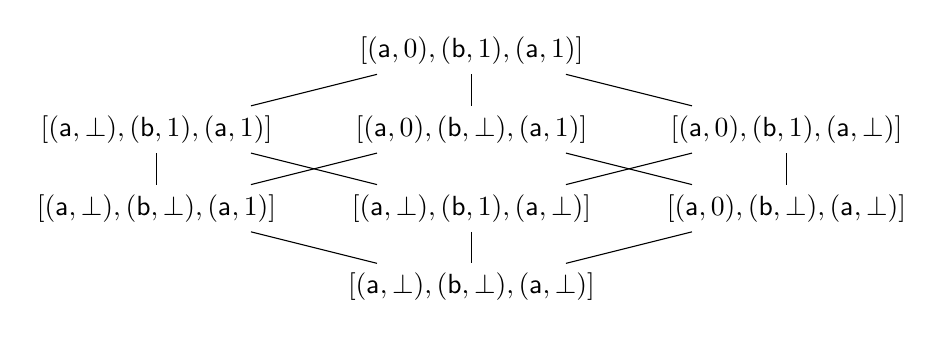
\begin{tikzpicture}
      \node (top) at (0,0) {$[(\mathsf{a}, 0), (\mathsf{b}, 1), (\mathsf{a}, 1)]$};
      % row 2
      \node [below of=top] (ioi) {$[(\mathsf{a}, 0), (\mathsf{b}, \bot), (\mathsf{a}, 1)]$};
      \node [left of=ioi,xshift=-3cm] (oii) {$[(\mathsf{a}, \bot), (\mathsf{b}, 1), (\mathsf{a}, 1)]$};
      \node [right of=ioi,xshift=3cm] (iio) {$[(\mathsf{a}, 0), (\mathsf{b}, 1), (\mathsf{a}, \bot)]$};
      % row 3
      \node [below of=ioi] (oio) {$[(\mathsf{a}, \bot), (\mathsf{b}, 1), (\mathsf{a}, \bot)]$};
      \node [left of=oio,xshift=-3cm] (ooi) {$[(\mathsf{a}, \bot), (\mathsf{b}, \bot), (\mathsf{a}, 1)]$};
      \node [right of=oio,xshift=3cm] (ioo) {$[(\mathsf{a}, 0), (\mathsf{b}, \bot), (\mathsf{a}, \bot)]$};
      % row 4
      \node [below of=oio] (bot) {$[(\mathsf{a}, \bot), (\mathsf{b}, \bot), (\mathsf{a}, \bot)]$};

      % links
      \draw (top) -- (ioi);
      \draw (top) -- (oii);
      \draw (top) -- (iio);
      \draw (ioi) -- (ooi);
      \draw (ioi) -- (ioo);
      \draw (oii) -- (ooi);
      \draw (oii) -- (oio);
      \draw (iio) -- (ioo);
      \draw (iio) -- (oio);
      \draw (ooi) -- (bot);
      \draw (oio) -- (bot);
      \draw (ioo) -- (bot);
    \end{tikzpicture}
  \end{center}
  The output approximation lattice looks like this, where $1$ is the actual data point that was returned in both runs of the program, and $\bot$ indicates that we are approximating this piece of data away:
  \begin{center}
    \begin{tikzpicture}
      \node (top) at (0,0) {$1$};
      \node [below of=top] (bot) {$\bot$};
      \draw (top) -- (bot);
    \end{tikzpicture}
  \end{center}
  These are not the only choices of approximation lattices that we could have taken. For the input, we have chosen a lattice that allows us to ``forget'' (approximate away) numbers in the input, but not any of the other data or the overall structure. However, other choices are also useful. Indeed, one of the aims of this work is to clarify how to choose an approximation structure appropriate for different tasks by use of type information. We elaborate on this further in Section \todo{XYZ}.

  Galois program slicing associates with each run of the program a Galois connection telling us how the inputs and outputs are related in that run. The backwards portion $\partial (\mathit{query}\,l)_r$ tells us, given an approximation of the output, what the least approximation of the input is needed to generate that output. In the case of the two runs considered in this example, if we say we are not interested in the output by feeding in the least approximation $\bot$, then we find that we only need the least approximation of the input:
  \begin{displaymath}
    \partial (\mathit{query}\,l)_r(\bot) = [(\mathsf{a},\bot), (\mathsf{b}, \bot), (\mathsf{a}, \bot)]
  \end{displaymath}
  for both $l = \mathsf{a}$ and $l = \mathsf{b}$. If instead we take the greatest approximation of the output (i.e., the output ``$1$'' itself), then the two query runs' backwards approximations return different results:
  \begin{displaymath}
    \begin{array}{l}
      \partial (\mathit{query}\,\mathsf{a})_r(1) = [(\mathsf{a},0), (\mathsf{b},\bot), (\mathsf{a},1)] \\
      \partial (\mathit{query}\,\mathsf{b})_r(1) = [(\mathsf{a},\bot), (\mathsf{b},1), (\mathsf{a},\bot)]
    \end{array}
  \end{displaymath}
  Pieces of the input that were {\em not} used are replaced by $\bot$. As we expect, the run of the query with label $\mathsf{a}$ depends on the entries in the database labelled with $\mathsf{a}$, and likewise for the run with label $\mathsf{b}$.

  In this case, the forwards portion of the Galois connection tells us for each approximation of the input whether or not it is sufficient to compute the output. In this example, if we provide insufficient data to compute the output, then we will get an underapproximated output. For example, $\partial (\mathit{query}\, \mathsf{a})_f([(\mathsf{a},0),(\mathsf{b},\bot),(\mathsf{a},\bot)]) = \bot$ because we need all the values associated with the label $\mathsf{a}$ to compute their sum.

  In a simple query like this, it is easy to work out the dependency relationship between the input and output. However, the benefit of Galois Program Slicing is that it is {\em automatic} for all programs, no matter how complex the relationship between input and output. Moreover, by changing what we mean by ``approximation'' we can compute a range of different information about a program.
\end{example}

Previous work on Galois program slicing uses an operational semantics of programs that generates a trace of each execution which can be interpreted after the fact to compute the Galois connection described above. This becomes {\em program slicing} by including the source code of the program as part of the input, so that, in the backward direction, the least approximation of the input required for an output approximation includes the least part of the program required.

\todo{Explain what the plan for the paper is}

\todo{Perhaps more elaboration on the applications of program slicing}

\subsection{Galois Program Slicing and Automatic Differentiation}

\todo{explain why we want a more abstract view on Galois program slicing}
There is a close analogy between Galois Program Slicing and Automatic Differentiation for differentiable programs. We have already hinted at this in the description above, but let us now make it explicit.

\begin{itemize}
\item For Galois Program Slicing, we assume that every value has an associated lattice of {\em approximations}. For differentiable programs, every point has an associated vector space of {\em tangents}.
\item For Galois Program Slicing, every program has an associated forward approximation map that takes approximations forward from the input to the output. This map {\em preserves meets}. For differentiable programs, every program has a forward derivative that takes tangents of the input to tangents of the output. The forward derivative map is {\em linear}, so it preserves addition of tangents and the zero tangent.
\item For Galois Program Slicing, every program has an associated backward approximation map that takes approximations of the output back to least approximations of the input. This map {\em preserves joins}. For differentiable programs, every program has a reverse derivative that takes tangents of the output to tangents of the input. This map is again {\em linear}.
\item For Galois Program Slicing, the forward and backward approximation maps are related by being a Galois connection. For differentiable programming, the forward and reverse derivatives are related by being each others' transpose.
\end{itemize}

Given this close connection between Galois program slicing and differentiable programming, we can take structures intended for modelling automatic differentiation and use them to model Galois program slicing. This will enable us to generalise and expand the scope of Galois program slicing to act as a foundation for data provenance in a wide range of computational settings.

\subsection{Outline and Contributions}

Our primary contribution in this article is to elucidate Galois Program Slicing by relating it to differentiable programming and automatic differentiation. In doing so, we aim to expand the applicability of program slicing, and to potentially transfer efficient automatic differentiation implementation techniques from automatic differentiation to program slicing and provenance tracking.

\begin{enumerate}
\item We explain how the CHAD framework of Vákár et al. can be adapted to give a general categorical framework for Galois Program Slicing,
\item Using our adapted CHAD framework, we can explain how type structure can be used to control the approximation lattices associated with data points, something that was ``hard coded'' in previous presentations of Galois Program Slicing.
\item With the benefit of our abstract setting, we can relate Galois Program Slicing to other parts of denotational semantics. In particular, we show that there is a close connection with Stable Domain Theory, a proposed solution to capturing sequentiality by recording more intensional information about programs' sensitivity to approximations.
\item We also relate Galois Program Slicing to categorical treatments of differentiability via Tangent Categories \note{Bob: not sure about this.}
\end{enumerate}

\section{Approximations as Tangents}
\label{sec:approx-as-tangents}

We motivate our approach to \GPS by showing how to combine ideas from differential geometry and stable domain theory to reconstruct \GPS in a denotational setting. From this basis, we apply the CHAD framework of V{\'a}k{\'a}r \etal to obtain a denotational model of automatic differentiation that gives us an effective way to interpret programs as functions along with their forward and backwards approximation maps.

\subsection{Manifolds, Smooth Functions, and Automatic Differentiation}
\label{sec:approx-as-tangents:autodiff}

% For what follows we do not need to know in detail what a manifold is, or exactly how smooth functions are defined. We only state some definitions in order to fix terminology and to justify our claim of a connection to manifolds and smooth functions. \bob{Need a good reference here.}

The general study of differentiable functions takes place on
\emph{manifolds}, topological spaces that ``locally'' behave like an
open subset of the Euclidean space $\RR^n$. The spaces $\RR^n$
themselves are manifolds, but so are ``non-flat'' examples such as
$n$-spheres and yet more exotic spaces. Every point $x$ in a manifold
$M$ has an associated \emph{tangent vector space} $\tangents_x(M)$
consisting of linear approximations of curves on the manifold passing
through $x$. Each point also has a \emph{cotangent vector space}
$\cotangents_x(M) = \tangents_x(M) \linearto \RR$. The tangent and
cotangent spaces are finite dimensional, so in the presence of a
chosen basis they are canonically isomorphic. In the case when the
manifold is $\RR^n$, then every tangent space is isomorphic to $\RR^n$
as well.

Smooth functions $f$ between manifolds $M$ and $N$ are functions on their points that are locally differentiable on $\RR^n$. Manifolds and smooth functions form a category $\Man$. Each smooth function induces maps of the (co)tangent spaces:
\begin{itemize}
\item The \emph{forward derivative} (tangent map, pushforward) $\pushf{f}_x$ is a linear map $\tangents_x(M) \linearto \tangents_{f(x)}(N)$. In the Euclidean case when $M = \RR^m$ and $N = \RR^n$, the tangent map can be represented by the Jacobian matrix of partial derivatives of $f$ at $x$.
\item The \emph{backward derivative} (cotangent map, pullback) $\pullf{f}_x$ is a linear map $\cotangents_{f(x)}(N) \linearto \cotangents_x(M)$. In the Euclidean case, the backward derivative is represented by the transpose of the Jacobian of $f$ at $x$.
\end{itemize}

\begin{remark}[Chain Rule]
  \label{rem:chain-rule}
  A useful property of derivative maps is that they compose according
  to the chain rule. Suppose that $f : M \to N$ and $g : N \to K$ are
  smooth functions. Then for any $x \in M$, we have:
  \begin{itemize}
  \item $\pushf{(g \circ f)}_x = \pushf{g}_{f(x)} \circ \pushf{f}_x : \tangents_x(M) \linearto \tangents_{g(f(x))}(K)$
  \item $\pullf{(g \circ f)}_x = \pullf{f}_x \circ \pullf{g}_{f(x)} : \cotangents_{g(f(x))}(K) \linearto \cotangents_x(M)$
  \end{itemize}
  The chain rule has the practical effect that we can compute
  derivative maps of $f$ and $g$ independently and compose them,
  instead of the potentially more difficult task of computing the
  derivative maps of $g \circ f$. As we shall see below, stable maps
  also obey a chain rule, and this forms the basis of the general
  categorical approach to differentiability that we describe in
  \secref{models-of-total-gps}.
\end{remark}

Computing the forward and backward derivatives of smooth functions $f$ has many applications of practical interest. For example, computation of the reverse derivative is of central interest in machine learning by gradient descent, the main technique used to train deep neural networks~\cite{rumelhart88,goodfellow16}.

Derivatives can be computed numerically by computing $f$ on small perturbations of its input, or symbolically by examining a closed-form representation of $f$. However, a more common and practical technique is to use \emph{automatic differentiation}, where a program computing $f$ is instrumented to produce (a representation of) the forward and/or backward derivative as a side-effect of producing the output~\cite{linnainmaa76}. This has led to the area of differentiable programming, where programming languages and their implementations are specifically designed to admit efficient automatic differentation algorithms~\cite{jax2018github,abadi16,elliott17,sigal24}.

\subsection{Stable Functions as Differentiable Functions}

Our thesis is that \GPS is a generalised form of differentiable programming, where tangents are not linear approximations of curves but instead are qualitative information approximations of elements. Smooth functions in this setting are Berry's \emph{stable functions} \cite{berry79,berry82}. We now introduce these concepts and how they relate to \GPS.

\subsubsection{Domains as a Qualitative Theory of Approximation}

Domain theory is a method for defining the semantics of programs that
handle infinite data such as functions or infinite streams. Domains
are certain partially ordered sets where the ordering denotes a
relationship of qualitative information content: if $x \sqsubseteq y$,
then $y$ may contain more information than $x$. For example, if $x$
and $y$ are functions, then $y$ may be defined at more values than
$x$. Infinite objects are understood in terms of their approximations
in this sense, and domains are assumed to be closed under least upper
bounds (lubs) of directed sets, meaning that any internally consistent
collection of elements has a ``completion'' that contains all the
information covered by the set. Programs are interpreted as monotone
functions that preserve directed lubs. Monotonicity captures the idea
that if the input gets more defined, then the output can get more
defined. Preservation of lubs, or \emph{continuity}, states that a
function interpreting a program cannot act inconsistently on
approximations and their completion, which corresponds to the
intuitive idea that a function that is computable cannot look at a
non-finite amount of input to produce a finite output. \citet{abramsky-jung} provide a comprehensive introduction to domain theory.

For the purposes of \GPS, we are interested in using
approximations not to model computation on infinite objects, but instead
for revealing how programs explore their inputs when producing parts
of their output. Therefore, we ignore completeness properties of the
partially ordered sets we consider\footnote{\bob{we might want to bring this back when considering general recursive programs. Are bidomains \cite{berry79} useful? they have two orderings. See also Laird's Bistable Biorders \cite{laird07}.}}.

\subsubsection{Bounded Meets and Conditional Multiplicativity}
\label{sec:bounded-meets-and-cm}

When giving a denotational semantics for sequential programming
languages, Scott-continuous functions are too permissive. Famously,
\citet{plotkin77lcf}'s Parallel OR (\exref{parallel-or}, below) is
continuous but does not explore its input in a way consistent with a
sequential implementation. Continuous functions can explore their
input in a non-deterministic way as long as the result is
deterministic. This non-determinism results in functions whose
output cannot be assigned a unique minimal input that accounts for
it. Therefore, continuous functions are incompatible with the central
idea in \GPS that we should be able to identify a \emph{minimal} part
of the input that leads to a part of the output.

\emph{Stability} is a property that can be required of monotone functions, that was invented by \citet{berry79} in an attempt to capture sequentiality. This was unsuccessful (see the $\mathrm{gustave}$ function in \exref{parallel-or}), but we will see now how it is closely related to the problem of computing forward and backwards maps of approximations needed in \GPS. A textbook description of stable functions in the context of domain theory is given by \citet[Chapter 12]{amadio-curien}. We start with a property that is weaker than stability, but is easier to motivate in connection with derivatives of smooth functions.

In a partially ordered set $X$, for any $x \in X$ the set of elements below $x$, $\downset{x} = \{ x' \mid x' \sqsubseteq x \}$, is itself a partially ordered set. These approximations of $x$ we will think of as ``tangents'' at $x$, and the whole set $\downset{x}$ as the ``tangent space''. Tangent spaces are vector spaces, so in the partially ordered setting we take elements of $\downset{x}$ to be approximations of processes defined at $x$. As we can add tangents, we assume we can take meets of approximations in $\downset{x}$:

% \footnote{\bob{Is it possible to derive the tangent spaces by
% thinking about continuous functions passing through $x$?}}

\begin{definition}
  A \emph{bounded meet poset} is a partially ordered set $X$ where for
  every $x \in X$, $\downset{x}$ is a meet semilattice, with $x$ as
  the top element.
\end{definition}

For the approximation version of the forward derivative of $f$ at $x$, we take $f$'s restriction to $\downset{x}$, taking approximations of the input to approximations of the output. Matching the linearity of the forward derivative of smooth functions, we require that these restrictions preserve meets. This is exactly the definition of \emph{conditionally multiplicative} function from \citet{berry79}:

\begin{definition}
  A \emph{conditionally multiplicative} (cm) function $f : X \to Y$ is
  a monotone function such that for all $x \in X$, the restriction
  $f_x : \downset{x} \to \downset{f(x)}$ preserves meets.
\end{definition}

\begin{theorem}
  Bounded meet lattices and conditionally multiplicative functions form
  a category $\CM$. This category has products, coproducts, and
  exponentials.
\end{theorem}

\begin{proof}
  \AGDA. See \citet[Theorem 12.2.8]{amadio-curien} for the
  case when the posets are also cpos. The crucial technical step,
  identified by \citet{berry79}, is that the ordering on conditionally
  multiplicative functions is not the extensional ordering
  ($f \sqsubseteq_{\mathrm{ext}} g$ iff
  $\forall x. f(x) \sqsubseteq g(x)$) but instead the stable ordering:
  $f \sqsubseteq_{\mathrm{st}} g$ iff $f \sqsubseteq_{\mathrm{ext}} g$ and
  $\forall x, x'.\,x \sqsubseteq x' \Rightarrow f(x) = f(x') \land
  g(x)$.
\end{proof}

\begin{remark}[Chain Rule]
  \label{rem:chain-rule-cm}
  It is almost a triviality at this point, but the crucial point is
  that, for any cm functions $f : X \to Y$ and $g : Y \to Z$, the
  restriction maps (``forward derivatives'') compose according to the
  chain rule from \remref{chain-rule}:
  \begin{displaymath}
    (g \circ f)_x = g_{f(x)} \circ f_x
  \end{displaymath}
  We will see this phenomenon repeated in the definition of stable
  functions below.
\end{remark}

\begin{example}[Conditionally Multiplicative Functions]
  \label{ex:strict-short-circuit}
  To see the effect of conditional multiplicativity, consider several
  ways of defining the OR on the lifted booleans
  $\mathbb{B}_\bot$. Two functions that are cm are the strict and
  left-short-circuiting ORs\footnote{The clauses in these examples are
    shorthand for the graph of the function. They are not to be
    understood as pattern matching clauses in a language like Haskell,
    where it is not possible to match on $\bot$.}:
  \begin{displaymath}
    \begin{array}[t]{l@{(}l@{,~}l@{)~}c@{~}l}
      \mathrm{strictOr}&\mathsf{tt}&\mathsf{tt}&=&\mathsf{tt} \\
      \mathrm{strictOr}&\mathsf{tt}&\mathsf{ff}&=&\mathsf{tt} \\
      \mathrm{strictOr}&\mathsf{ff}&\mathsf{tt}&=&\mathsf{tt} \\
      \mathrm{strictOr}&\mathsf{ff}&\mathsf{ff}&=&\mathsf{ff} \\
      \mathrm{strictOr}&\bot&\_&=&\bot \\
      \mathrm{strictOr}&\_&\bot&=&\bot \\
    \end{array}
    \qquad
    \begin{array}[t]{l@{(}l@{,~}l@{)~}c@{~}l}
      \mathrm{shortCircuitOR}&\mathsf{tt}&\_&=&\mathsf{tt} \\
      \mathsf{shortCircuitOR}&\mathsf{ff}&x&=&x \\
      \mathsf{shortCircuitOR}&\bot&\_& =& \bot
    \end{array}
    \qquad
    \raisebox{-15ex}{
      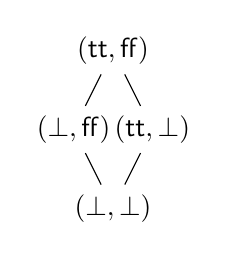
\begin{tikzpicture}
        \node (top) at (0,0) {$(\mathsf{tt},\mathsf{ff})$};
        \node [below of=top,xshift=-0.5cm] (oi) {$(\bot,\mathsf{ff})$};
        \node [below of=top,xshift=0.5cm] (io) {$(\mathsf{tt},\bot)$};
        \node [below of=oi,xshift=0.5cm] (oo) {$(\bot,\bot)$};
        \draw (top) -- (oi);
        \draw (top) -- (io);
        \draw (oi) -- (oo);
        \draw (io) -- (oo);
      \end{tikzpicture}
    }
  \end{displaymath}
  In the poset $\mathbb{B}_\bot^2$, a typical poset of approximations of a fully defined element is shown to
  the right. For $\mathrm{strictOr}$, any approximation that isn't the fully defined input is mapped to
  $\bot$, while $\mathrm{shortCircuitOr}$ maps the partially defined $(\mathsf{tt},\bot)$ to $\mathsf{tt}$.
  Thus, even though these functions operate identically on fully defined inputs, they differ in their
  \emph{derivatives} on partially defined input, exposing how they explore their arguments differently. That
  they are cm can be checked by examining their restrictions' behaviour. If we take the approximations
  $(\bot,\mathsf{ff})$ and $(\mathsf{tt},\bot)$, then their meet is $(\bot,\bot)$; $\mathrm{strictOr}$ maps
  all three elements to $\bot$, so is cm here since $\bot \wedge \bot = \bot$; and $\mathrm{shortCircuitOR}$
  has $(\bot,\mathsf{ff}) \mapsto \bot$ and $(\mathsf{tt},\bot) \mapsto \mathsf{tt}$, the meet of which is
  $\bot = \mathrm{shortCircuitOR}(\bot,\bot)$. Other combinations can be checked similarly.
\end{example}

\begin{example}[A non-Conditionally Multiplicative Function]
  \label{ex:parallel-or}
  A function that is not cm is Plotkin's Parallel OR \cite{lcf77}, which short-circuits in both arguments. It returns $\mathsf{tt}$ if either argment is $\mathsf{tt}$ even if the other argument is not defined:
  \begin{displaymath}
    \begin{array}{l@{(}l@{,~}l@{)~}c@{~}l}
      \mathrm{parallelOR}&\mathsf{tt}&\_&=&\mathsf{tt} \\
      \mathrm{parallelOR}&\_&\mathsf{tt}&=&\mathsf{tt} \\
      \mathsf{parallelOR}&\mathsf{ff}&\mathsf{ff}&=&\mathsf{ff} \\
      \mathsf{parallelOR}&\bot&\bot&=&\bot
    \end{array}
  \end{displaymath}
  We have $\mathrm{parallelOR}(\mathsf{tt}, \bot) \wedge \mathrm{parallelOR}(\bot, \mathsf{tt}) = \mathsf{tt} \wedge \mathsf{tt} = \mathsf{tt}$ but $\mathrm{parallelOR}((\mathsf{tt},\bot) \wedge (\bot, \mathsf{tt})) = \mathrm{parallelOR}(\bot, \bot) = \bot$, so it is not cm.

  Parallel OR is famous because it is not \emph{sequential}, meaning intuitively that it cannot be implemented without running the two arguments in parallel to see if one of them returns $\mathsf{tt}$. The fact that it exists in the standard domain theoretic semantics of PCF means that this semantics is incomplete for reasoning about observational equivalence in PCF. Since Parallel OR is not cm, one might hope that cm-ness is enough to capture sequentiality, and hence potentially give a fully abstract model of PCF. However, the following ternary function $\mathbb{B}_\bot^3 \to \{\top,\bot\}$ is cm but admits no sequential implementation that fixes an order that the arguments are examined in:
  \begin{displaymath}
    \begin{array}{l@{(}l@{,~}l@{,~}l@{)~}c@{~}l}
      \mathrm{gustave}&\mathsf{tt}&\mathsf{ff}&\_&=&\top \\
      \mathrm{gustave}&\mathsf{ff}&\_&\mathsf{tt}&=&\top \\
      \mathrm{gustave}&\_&\mathsf{tt}&\mathsf{ff}&=&\top \\
      \mathrm{gustave}&\_&\_&\_&=&\bot
    \end{array}
  \end{displaymath}
  Due to the way that the cases are defined, there is no way of constructing a pair of approximations for which preservation of their meet does not hold. In terms of derivatives, this makes sense in that we are only concerned about the intensional behaviour of a function at a point and its approximations. Parallel OR has two incompatible approximation behaviours at the point $(\mathsf{tt},\mathsf{tt})$. The $\mathrm{gustave}$ function does have consistent behaviour at each approximation for each point.
\end{example}

\begin{example}[Intervals and Maximal Elements]
  \label{ex:intervals-and-maxima-elements}
  The set of intervals
  $\{ [l,u] \in \mathbb{R} \times \mathbb{R} \mid l \leq u \}$ ordered
  by reverse inclusion forms a (Scott) domain
  \cite{scott-outline}. The set of maximal elements is exactly
  $\mathbb{R}$. This domain has been proposed as a model of
  approximate real number computation \cite{escardo-real-pcf}. The
  information approximation reading is intuitive: as intervals move up
  the order they become tighter, containing more information about the
  number they are approximating.

  Given this reading, it makes sense to wonder if we can use interval
  approximations as ``information tangents'' of real numbers, where
  derivatives take approximating intervals to approximating
  intervals. Since intervals form a Scott domain, they are bounded
  complete and hence have bounded meets. However, the addition
  function on intervals, $[l_1,u_1] + [l_2,u_2] = [l_1+l_2,u_1+u_2]$,
  is not conditionally multiplicative, as can be easily checked.

  A solution is to use the set of intervals with nominated points that
  they are approximating: $\{[l,x,u] \mid l \leq x \leq u\}$. The
  ordering now is that $[l_1,x_1,u_1] \sqsubseteq [l_2,x_2,u_2]$ iff
  $x_1 = x_2$ and $l_1 \leq l_2$ and $u_2 \leq u_1$. Consequently, the
  maximal elements are $[x,x,x]$, recovering $\mathbb{R}$ again, but
  the approximations of each number all form independent sub-lattices.
  Addition is defined as
  $[l_1,x_1,u_1] + [l_2,x_2,u_2] = [(l_1+x_2) \sqcap
  (l_2+x_1),x_1+x_2,(u_1+x_2)\sqcup(u_2+x_1)]$, which is conditionally
  multiplicative. Note how this definition bears a resemblance to the
  product rule for derivatives, with (in the lower end of the
  interval) $\sqcap$ replacing $+$.

  This example is important to us because it shows that (for total
  programs) we are separately interested in the maximal elements and
  their approximations, and that approximations of each maximal
  element may have to be considered separately.

  Relatedly, \citet{edalat-heckmann98} proposed a Scott domain of
  formal balls on a metric space, where again the maximal elements are
  the points of the original space. More generally,
  \citet[Section V-6]{continuous-lattice-book} describe \emph{domain
    environments}, which are domains whose maximal elements are
  exactly the points of a topological space. We are not aware of any
  work linking domain environments in general to stable functions. It
  would be interesting to see whether the situation for intervals,
  where approximations must be relative to a nominated point, repeats
  in general when considering conditionally multiplicative functions.
\end{example}

Given these examples, conditional multiplicativity seems to be a
reasonable analogue to functions with a well-defined notion of
derivative. For \GPS we also require an analogue to the reverse
derivative, where we map approximations backwards to give the least
approximation of the input for a given approximation of the output. In
the case of smooth functions, we are always guaranteed a reverse
derivative. However, there is not always a best way to map
approximations backwards for cm functions, as the following example
shows.

\begin{example}[Is Conditional Multiplicativity Enough?]
  \label{ex:non-stable-function}
  An example that is conditionally multiplicative, but does not admit
  a backwards map of approximations (from \citet[just
  before Lemma 12.2.3]{amadio-curien}, originally due to Berry) is given by defining
  $\mathrm{unstable} : D \to \{\bot \sqsubseteq \top\}$, where
  $D = \bot \sqsubseteq \cdots \sqsubseteq n \sqsubseteq \cdots
  \sqsubseteq 1 \sqsubseteq 0$, as $\mathrm{unstable}(\bot) = \bot$
  and $\mathrm{unstable}(n) = \top$. This is monotone, and preserves
  meets in every $\downset{x}$. However, there is no ``best'' (i.e.,
  least) input that gives us any finite output.
\end{example}

\subsubsection{Stable functions and L-posets}
\label{sec:stab}

In light of the \exref{non-stable-function}, we turn to
\citet{berry79}'s definition of \emph{stable function} that requires
the existence of a reverse mapping directly, even without assuming
that any meets exist:

\begin{definition}[Stable function]
  Let $f : X \to Y$ be a monotone function between posets $X$ and
  $Y$. The function $f$ is \emph{stable} if for all $x \in X$ and
  $y \leq f(x)$:
  \begin{enumerate}
  \item (\textsc{Existence}) there exists an $x_0 \leq x$ such that $y \leq f(x_0)$, and
  \item (\textsc{Minimality}) for any $x'_0 \leq x$ such that $y \leq f(x'_0)$ then
    $x_0 \leq x'_0$ .
  \end{enumerate}
\end{definition}

\begin{example}\label{ex:stable-functions}
  \leavevmode\\[-3ex]
  \begin{enumerate}
  \item The function $\mathrm{strictOr}$ is stable. For example, for
    the input-output pair
    $(\mathsf{tt},\mathsf{ff}) \mapsto \mathsf{tt}$, the minimal input
    that gives this output is exactly $(\mathsf{tt}, \mathsf{ff})$. If
    we take the approximation $\bot \leq \mathsf{tt}$ of the output,
    then the corresponding minimal input is $(\bot, \bot)$. The
    function $\mathrm{shortCircuitOR}$ is also stable. For the
    input-output pair $(\mathsf{tt},\mathsf{ff}) \mapsto \mathsf{tt}$,
    the minimal input that gives this input is $(\mathsf{tt},\bot)$,
    indicating that the presence of $\mathsf{ff}$ in the second
    argument was not necessary to produce this output. As with
    $\mathrm{strictOr}$, the minimal input required to produce the
    output $\bot \leq \mathsf{tt}$ is again $(\bot,\bot)$.

  \item The $\mathrm{parallelOR}$ function is not stable. For the
    input-output pair $(\mathsf{tt},\mathsf{tt}) \mapsto \mathsf{tt}$,
    there is no one minimal input that produces this output. We have
    both $\mathrm{parallelOR}(\mathsf{tt},\bot) = \mathsf{tt}$ and
    $\mathrm{parallelOR}(\bot,\mathsf{tt}) = \mathsf{tt}$, which are
    incomparable and their greatest lower bound $(\bot,\bot)$ gives
    the output $\bot$.

  \item The $\mathrm{gustave}$ function is stable. Despite there being
    no one minimal input that achieves the output $\top$, each of the
    minimal inputs that can achieve this output are pairwise
    incomparable, so for each specific input that gets output $\top$
    there is a unique minimal input that achieves it (listed in the
    first three lines of the definition).

    In terms of \GPS the $\mathrm{gustave}$ function does not present
    a problem. For any particular run (i.e., input $\mapsto$ output
    pair), there is an unambiguous minimal input that achieves the
    output, no matter that it was not achieved by a sequential
    processing of the input.

  \item As discussed above, $\mathrm{unstable}$ is not stable, but is
    conditionally multiplicative.

  \item The addition function on intervals with nominated points in
    \exref{intervals-and-maxima-elements} is stable. Given the input
    $[l_1,x_1,u_1], [l_2,x_2,u_2]$ and an approximation
    $[l,x_1+x_2,u]$ of the output, the minimal approximations of the
    input are $[l-x_2,x_1,u-x_2], [l-x_1,x_2,u-x_1]$. We can read this
    as saying if the output was the maximal element $x_1+x_2$ but we
    only require the output to be in the range $[l,x_1+x_2,u]$, then
    we can obtain intervals containing the input values that are
    enough to obtain the desired output approximation \emph{assuming
      that the other input is kept the same}. Note the analogy to
    partial derivatives in multi-variable calculus, where the
    derivative is computed in each variable independently.
  \end{enumerate}
\end{example}

% The fact that these two functions' stability witnesses reveal
% information about how they depend on their input is what we will
% exploit in order to use the idea of stability for \GPS. It is
% interesting that sequentiality is not necessarily required in order
% to obtain backwards maps of approximations, as might be assumed by
% thinking about how to trace computations for provenance information.

Stability has an alternative definition in terms of Galois
connections, which will be more useful for what follows. This
characterisation is due to~\citet{taylor99}. We first define Galois
connections, which we used informally in \exref{introduction-example}.

\begin{definition}[Galois connection]
  \label{def:galois-connection}
  Suppose $X$ and $Y$ are posets. A \emph{Galois connection} $f \adj g: X \to Y$ is a pair of monotone functions $f: Y \to X$ and $g: X \to Y$ satisfying $y \leq g(x) \iff f(y) \leq x$ for any $x \in X$ and $y \in Y$. Since a Galois connection is also an adjunction, we refer to $f$ as the left adjoint and $g$ as the right adjoint.
\end{definition}

\begin{lemma}
  A monotone function $f : X \to Y$ is stable if and only if for all
  $x \in X$, the restriction of $f_x : \downset{x} \to \downset{f(x)}$
  has a left Galois adjoint.
\end{lemma}

\begin{proof}
  If $f$ is stable, then define a left adjoint
  $f^*_x : \downset{f(x)} \to \downset{x}$ by setting $f^*_x(y)$ to be
  the minimal $x_0$ required by stability. This is monotone: if
  $y \leq y'$, then we know that $y \leq y' \leq f(f^*_x(y'))$ by
  definition of $f^*_x$, so $f^*_x(y) \leq f^*_x(y')$ by minimality of
  $f^*_x(y)$. For the adjointness, let $x' \leq x$ and $y \leq
  f(x)$. Then if $f^*_x(y) \leq x'$, we have
  $y \leq f(f^*_x(y)) \leq f(x')$ by monotonicity of $f$ and the first
  part of stability. In the other direction, if we have
  $y \leq f(x')$, then by uniqueness we have $f^*_x(y) \leq x'$.

  If, for every $x$, $f_x$ has a left adjoint $f^*_x$, then for any
  $x', y$ we have $y \leq f_x(x') \Leftrightarrow f^*_x(y) \leq
  x'$. So $f^*_x(y)$ is the element that satisfies
  $y \leq f(f^*_x(y))$, and it is minimal since if $y \leq f_x(x'_0)$
  then $f^*_x(y) \leq x'_0$.
\end{proof}

Even though stable functions can be defined on any partially ordered
set, in light of the analogy with tangent spaces it makes sense to
require that meets, preserved by forward approximation maps, and
joins, preserved by backwards approximation maps, exist:

\begin{definition}
  An \emph{L-poset} is a partially ordered set $X$ such that for every $x \in X$, the principal downset $\downset{x}$ is a bounded lattice (i.e., have all finite meets and joins).
\end{definition}

This lemma is an instance of standard facts about Galois connections
preserving meets and joins:

\begin{lemma}
  For L-posets $X$ and $Y$, a stable function $f : X \to Y$ preserves
  meets in its forward part $f_x$ and joins in its reverse part
  $f^*_x$.
\end{lemma}

The converse to this lemma (that functions that preserve meets in their forward part have a left Galois adjoint) is not true, as was demonstrated by the non-stable function in \exref{non-stable-function}. In the case when the posets $\downset{x}$ are \emph{complete}, and $f_x$ preserves infinitary meets, then we are guaranteed a left Galois adjoint. In that example, the infinite set $\{0, 1, 2, \dots, n, n-1, \dots\}$ not including $\bot$ of approximations of $0$ does not have a greatest lower bound, so the order is not complete.

\begin{theorem}
  L-posets and stable functions form a category $\Lposet$ with products
  and coproducts.
\end{theorem}

\begin{remark}[Chain Rule]
  \label{rem:chain-rule-stable}
  As for the ``forward derivatives'' of conditionally multiplicative
  functions, the forward and backwards parts of a stable function
  compose according to the chain rule (c.f. \remref{chain-rule}):
  \begin{itemize}
  \item $(g \circ f)_x = g_{f(x)} \circ f_x : \downset{x} \linearto \downset{g(f(x))}$
  \item $(g \circ f)^*_x = f*_x \circ g^*_{f(x)} : \downset{g(f(x))} \linearto \downset{x}$
  \end{itemize}
  We will use this property in \propref{embed-stable} to show that
  $\Lposet$ embeds into our category of sets-with-approximation.
\end{remark}

The category of L-posets and stable functions is not cartesian
closed. To make it so, we would need to require that the principal
downsets $\downset{x}$ are \emph{complete}
lattices. \citet[Theorem 12.FIXME]{amadio-curien} details the
proof. Intuitively, to generate the best approximation of an input
value for a function, we need to take the infimum over all possible
input values.

Our goal is to model a higher-order language suitable for writing
queries on databases as in \exref{introduction-example}, so why should
we not just take complete L-posets and stable functions as our model
of \GPS?  We have two reasons for moving to a different model in
\secref{models-of-total-gps}:

\begin{enumerate}
\item Even without completeness, in Bounded meet posets and L-posets,
  values and their approximations live in the same set. However, in
  the \emph{total} query language we wish to model in
  \secref{language}, we are not directly interested in the behaviour
  of programs on approximations as we would be for partial programs
  with general recursion. (Moreover, in the light of
  \exref{intervals-and-maxima-elements} it is not clear whether
  approximations for partiality and approximations for stability ought
  to be the same thing. We discuss this further in
  \secref{conclusion}.) In \exref{intervals-and-maxima-elements},
  maximal elements could be taken to be the ``proper values''. One
  idea is to restrict to conditionally multiplicative or stable
  functions that preserve maximal elements. However, this idea fails
  at higher order: functions that take maximal elements to maximal
  elements are not themselves maximal elements. We could devise a
  category of L-posets with totality predicates (which would pick out
  maximal elements at first-order) and totality preserving functions,
  but we prefer a more direct method of separating values proper from
  their approximations using the \emph{Category of Families}
  construction we detail in \secref{models-of-total-gps:fam}.
\item A more practical reason is that we wish to formalise our
  construction in the proof assistant Agda \cite{agda} in order to get
  an \emph{executable} model of the language in
  \secref{language}. Agda's type theory is both predicative and
  constructive. Predicativity means that it does not have complete
  lattices in the classical sense: for a type $X$ we can only get
  suprema and infinma of families in a lower universe level than
  $X$. This is not necessarily a problem, as \citet{dejong21} shows
  how to develop a large amount of domain theory in a predicative
  setting. However, due to constructivity the lifting construction
  (due to \citet{escardo-knapp}) requires a proof of definedness to
  extract a value. Since we are modelling a total language, we prefer
  to have a model that computes directly.
\end{enumerate}

\subsection{Summary}
\label{sec:diff-stab-summary}

We have seen that \citet{berry79}'s theory of stable functions between suitable partial orders can be seen as form of differentiability with forward and reverse derivatives. In the next section, we describe a model based on these ideas suitable for constructing executable models of total higher order languages.

We end this section with a conjecture. Although we have argued above
that there is an analogy between stable functions and smooth
functions, we have not stated any mathematical theorems substantiating
this. \emph{Tangent Categories} \cite{cockett14,cockett18} are a
categorical axiomatisation of the properties of manifolds and smooth
functions in terms of the presence of tangent bundles $TX$ for every
object $X$, forward derivatives and additivity of tangents. They
generalise Cartesian Differential Categories \cite{cdcs}, which are an
axiomatisation of Euclidean spaces and smooth functions.

\begin{conjecture}
  \label{con:tangent-stable-fns}
  (1) Bounded meet posets and conditionally multiplicative functions
  form a Tangent category where the tangent bundle
  $TX = \{(x,x') \mid x' \leq x\}$ and addition of tangents is given
  by meets. (2) L-posets and stable functions form a \emph{reverse
    Tangent category} \cite{reverse-tangents}.
\end{conjecture}

As well as codifying exactly what we mean by differentiable structure
on partially ordered sets, proving this conjecture would also tell us
what higher derivatives mean in this context as well, something that
we have not considered above. We will extend this conjecture to our
refined model of lattice approximated sets in \secref{model-summary}.

% Let us summarise our analogy between differentiable functions between manifolds and stable functions between L-posets:

% \begin{itemize}
% \item For \GPS, we assume that every value has an associated lattice of {\em approximations}. For differentiable programs, every point has an associated vector space of {\em tangents}.
% \item For \GPS, every program has an associated forward approximation map that takes approximations forward from the input to the output. This map {\em preserves meets}. For differentiable programs, every program has a forward derivative that takes tangents of the input to tangents of the output. The forward derivative map is {\em linear}, so it preserves addition of tangents and the zero tangent.
% \item For \GPS, every program has an associated backward approximation map that takes approximations of the output back to least approximations of the input. This map {\em preserves joins}. For differentiable programs, every program has a reverse derivative that takes tangents of the output to tangents of the input. This map is again {\em linear}.
% \item For \GPS, the forward and backward approximation maps are related by being a Galois connection. For differentiable programming, the forward and reverse derivatives are related by being each others' transpose.
% \end{itemize}

\section{Models of Galois Slicing for a Total Language} % \GPS doesn't use title caps
\label{sec:models-of-total-gps}

The previous section concluded that L-posets and stable functions give
a model of \GPS analogous to manifolds and smooth functions. However,
we noted a conceptual shortcoming of this model, for the purposes of
modelling total computations, that proper values and their
approximations live in the same category. In this section, we propose
a model for total \GPS based on the \emph{Category of Families}
construction. This construction, and the more general Grothendieck
construction, has been previously used by V{\'a}k{\'a}r and
collaborators \cite{vakar22} to model automatic differentiation for
higher-order programs on the reals. We reuse some of their results,
and discuss the commonalities as we go.

\subsection{The Category of Families Construction}
\label{sec:models-of-total-gps:fam}

L-posets are partially ordered sets where every principal downset
$\downset{x}$ is a bounded lattice of approximations/tangents. As we
explained in \secref{stab}, the shortcoming of this setup is that
proper values and their approximations live in the same set. We fix
this by changing our model to one where we have sets $X$ of values,
and for each $x \in X$, a bounded lattice $\partial X(x)$ of
approximations of $x$. This construction is an instance of the general
\emph{Category of Families} construction:

\begin{definition}
  Let $\cat{C}$ be a category. The \emph{Category of Families} over
  $\cat{C}$, $\Fam(\cat{C})$, has as objects pairs $(X, \partial X)$,
  where $X$ is a set and $\partial X : X \to \cat{C}$ is an
  $X$-indexed family of objects in $\cat{C}$. A morphism
  $f : (X, \partial X) \to (Y, \partial Y)$ consists of a pair of a
  function $f : X \to Y$ and a family of morphisms of $\cat{C}$,
  $\partial f : \Pi_{x : X}.\,\cat{C}(\partial X(x), \partial Y(f\,x))$.
\end{definition}

The reason for choosing the $\Fam$ construction is that composition in
this category is an abstract version of the chain rule that we have
seen in \remref{chain-rule}, \remref{chain-rule-cm}, and
\remref{chain-rule-stable}. Composition $f \circ g $ of morphisms
$f : (Y, \partial Y) \to (Z, \partial Z)$ and
$g : (X, \partial X) \to (Y, \partial Y)$ in this category is given by
normal function composition on the set components, and
$\partial (f \circ g)(x) = \partial f(f, x) \circ \partial g(x)$,
where the latter composition is in $\cat{C}$.

The fact that morphisms in $\Fam(C)$ compose according to a chain rule
means that the categories we considered in \secref{approx-as-tangents}
embed into $\Fam(C)$ for appropriate $C$. If we let $\FinVect$ be the
category of finite dimensional real vector spaces and linear maps,
then:

\begin{proposition}
  \label{prop:embed-manifolds}
  There is a faithful functor $\Man \to \Fam(\FinVect)$ that sends a
  manifold $M$ to $(M, \lambda x. T_x(M))$, and each smooth function
  $f$ to $(f, f_*)$, the pair of $f$ and its forward derivative.
\end{proposition}

As similar result is given by \citet{cruttwell2022}, where Euclidean
spaces $\RR^n$ and smooth functions are embedded into a category of
lenses (the ``simply typed'' version of the $\Fam$ construction). As
in \citet{vakar22}, the idea is to formally separate functions on
points and their forward/reverse tangent maps for the purposes of
implementation of automatic differentiation. In the case of smooth
maps, this process throws away information on higher derivatives by
turning smooth maps into pairs of plain functions and linear
functions. We conjecture at the end of this section that the analogous
construction in our partially ordered setting does not.

For the categories $\CM$ and $\Lposet$, we pick the appropriate
categories of partial orders and monotone maps:

\begin{enumerate}[leftmargin=\enummargin]
\item The category $\LatGal$ has bounded lattices as objects and
  Galois connections as morphisms, with the right adjoint going in the
  ``forward'' direction. The category $\Fam(\LatGal)$ is our preferred
  model for total functions with Galois slicing. We explore some
  specific examples in this category in \secref{semantic-gps}.
\item The category $\MeetSLat$ has meet-semilattices with top as
  objects and monotone finite meet preserving functions as
  morphisms. The category $\Fam(\MeetSLat)$ provides a model of
  total functions with ``forward derivatives'' only.
\item The category $\JoinSLat$ has join-semilattices with bottom as
  objects and monotone finite join preserving functions as
  morphisms. The category $\Fam(\JoinSLat^\op)$ provides a model of
  total functions with ``backwards derivatives'' only.
\end{enumerate}

We can get an analogous result to \propref{embed-manifolds} for
L-posets and stable maps:

\begin{proposition}
  \label{prop:embed-stable}
  There is a faithful functor $\Lposet \to \Fam(\LatGal)$ that maps an
  L-poset $X$ to $(X, \lambda x. \downset{x})$ and stable functions
  $f$ to $(f, \lambda x. (f_x, f^*_x))$. Likewise, there is a faithful
  functor $\CM \to \Fam(\MeetSLat)$.
\end{proposition}

Despite its similarity, this proposition has a lesser status than
\propref{embed-manifolds} because it is not clear that the category
$\Lposet$ (or $\CM$) is a canonical definition of approximable sets
and functions with approximation derivatives, as we discussed at the
end of \secref{stab}.
% We could restrict $\Lposet$ to morphisms that preserve maximal
% elements and take L-posets $X$ to
% $(\mathrm{Max}(M), \lambda x. \downset{x})$.
Our working hypothesis is that $\Fam(\LatGal)$, where values and their
approximations are separated by construction, is a natural model of
semantic \GPS in a total setting, though we note some shortcomings in
\remref{further-structure}. We now investigate some categorical
properties of this category, with a view to modelling a higher-order
total programming language in \secref{language}.

\subsection{Categorical Properties of $\Fam(\cat{C})$}

\subsubsection{Coproducts and Products}
\label{sec:models-of-total-gps:coproducts-and-products}

The categories $\Fam(\cat{C})$ are the free coproduct completions of
categories $\cat{C}$, so they have all coproducts:

\begin{proposition}
  For any $\cat{C}$, $\Fam(\cat{C})$ has all coproducts, which can be
  given on objects by:
  \begin{displaymath}
    \coprod_i (X_i, \partial X_i) = (\coprod_i X_i, \lambda (i, x_i).\, \partial X_i(x))
  \end{displaymath}
  Coproducts in $\Fam(\cat{C})$ are \emph{extensive}
  \cite[Proposition 2.4]{carboni-lack-walters93}.
\end{proposition}

For $\Fam(\cat{C})$ to have finite products, we need $\cat{C}$ to have
finite products:

\begin{proposition}
  If $\cat{C}$ has finite products, then so does $\Fam(\cat{C})$. On
  objects, binary products can be defined by:
  \begin{displaymath}
    (X, \partial X) \times (Y, \partial Y) = (X \times Y, \lambda (x, y). \partial X(x) \times \partial Y(y))
  \end{displaymath}
  Since $\Fam(\cat{C})$ is extensive, products and coproducts
  distribute.
\end{proposition}

Using the infinitary coproducts and finite products, we can construct
a wide range of other useful semantic models of datatypes in
$\Fam(\cat{C})$. For example, lists can be constructed as a coproduct
\begin{equation}
  \label{eqn:lists}
  \List(X) = \coprod_{n \in \mathbb{N}} X^n
\end{equation}
where $X^0 = 1$ (the terminal object) and $X^{n+1} = X \times X^n$.

Our category of interest, $\Fam(\LatGal)$ has coproducts and finite
products, because $\LatGal$ has products. Similarly for
$\Fam(\MeetSLat)$. As we shall see below, the products in $\LatGal$
(and $\MeetSLat$ and $\JoinSLat)$ are also coproducts, which is
essential to obtaining cartesian closure.

\subsubsection{Cartesian Closure}

For cartesian closure of the categories $\Fam(C)$ that we are
interested in, we rely on the following theorem of \citet{nunes2023},
specialised from their setting with the general Grothendieck
construction to $\Fam(\cat{C})$. This relies on the definition of
\emph{biproducts}, which we discuss below in \secref{biproducts}.

\begin{theorem}[\cite{nunes2023}]
  \label{thm:fam-closed}
  \AGDA.  If $\cat{C}$ has biproducts (\defref{biproducts}) and all
  products, then $\Fam(\cat{C})$ is cartesian closed\footnote{More
    precisely, if $\cat{C}$ has coproducts then we have a monoidal
    product on $\Fam(\cat{C})$ which is closed by this
    construction. When these coproducts are in fact biproducts, we get
    cartesian closure.}. On objects, the internal hom can be given by:
  \begin{displaymath}
    (X, \partial X) \to (Y, \partial Y) = (\Pi_{x : X}. \Sigma_{y : Y}. \cat{C}(\partial X(x), \partial Y(y)), \lambda f. \Pi_{x : X}. \partial Y(\pi_1(f\, x)))
  \end{displaymath}
\end{theorem}

The $\Set$-component of $(X, \partial X) \to (Y, \partial Y)$ consists
of exactly the morphisms of $\Fam(\cat{C})$, rephrased into a single
object. When $\cat{C} = \FinVect$, these are functions with an
associated linear map at every point, and when $\cat{C} = \LatGal$,
these are functions with an associated Galois connection at every
point. A tangent to a function is then defined to be a mapping from
points in the domain to tangents in the codomain along the function.

The category $\MeetSLat$ satisfies the hypoetheses of
\thmref{fam-closed}, so:
\begin{corollary}
  $\Fam(\MeetSLat)$ is cartesian closed and has all coproducts.
\end{corollary}
Unfortunately, neither of the $\LatGal$ or $\FinVect$ satisfy the
hypotheses of this theorem, because neither of them have infinite
products. We will consider ways to rectify this below in
\secref{fixing-completeness}.

\begin{remark}
  \label{rem:hermida-exponentials}
  There is another construction of internal homs on $\Fam(\cat{C})$
  arising from the use of fibrations for categorical logical
  relations, due to \citet[Corollary 4.12]{hermida99}. If we assume
  that $\cat{C}$ is itself cartesian closed and has all products, then
  we could construct an internal hom as:
  \begin{displaymath}
    (X, \partial X) \to (Y, \partial Y) = (X \to Y, \lambda f. \Pi_{x : X}.\,\partial X(x) \to \partial Y(f\,x))
  \end{displaymath}
  However, for the purposes of modelling differentiable programs, this
  is fatally flawed in that neither of $\LatGal$ nor $\FinVect$ are
  cartesian closed, and there is no way of making them so without
  losing the property of being able to conjunct or add tangents, as we
  shall see below. We will implicitly use Hermida's construction in
  our definability proof in \secref{definability}, where we use a
  logical relations argument to show that every morphism definable in
  the higher order language is also first-order definable.
\end{remark}

\subsubsection{CMon-Categories and Biproducts}
\label{sec:biproducts}

Loosely stated, biproducts are objects that are both products and
coproducts. The concept can be defined in any category, as shown by
\citet{karvonen20}, but for our purposes it will be more convenient to
use the shorter definition in categories enriched in commutative
monoids:
\begin{definition}
  A category $\cat{C}$ is enriched in $\CMon$, the category of
  commutative monoids, if every homset $\cat{C}(X,Y)$ is a commutative
  monoid with $(+,0)$ and composition is bilinear:
  \begin{displaymath}
    f \comp \zero = 0 = \zero \comp f
  \end{displaymath}
  \begin{displaymath}
    (f + g) \comp h = (f \comp h) + (g \comp h) \qquad
    h \comp (f + g) = (h \comp f) + (h \comp g)
  \end{displaymath}
\end{definition}
In any $\CMon$-category we can define what it means to be the
biproduct of two objects:
\begin{definition}
  \label{def:biproducts}
  In a $\CMon$-category a biproduct is an object $X \biprod Y$
  together with morphisms

  \begin{center}
    \begin{tikzcd}
      X \arrow[r, "\biinj_X", shift left] &
      X \biprod Y \arrow[l, "\biproj_X", shift left] \arrow[r, "\biproj_Y"', shift right] &
      Y \arrow[l, "\biinj_Y"', shift right]
    \end{tikzcd}
  \end{center}

  \vspace{-1mm}
  \noindent satisfying

  \vspace{-5mm}
  \begin{minipage}[t]{0.45\textwidth}
    \begin{center}
      \begin{salign*}
        \biproj_X \comp \biinj_X &= \id_X \\
        \biproj_Y \comp \biinj_X &= \zero_{X,Y}
      \end{salign*}
    \end{center}
  \end{minipage}%
  \begin{minipage}[t]{0.45\textwidth}
    \begin{center}
      \begin{salign*}
        \biproj_Y \comp \biinj_Y &= \id_Y \\
        \biproj_X \comp \biinj_Y &= \zero_{Y,X}
      \end{salign*}
    \end{center}
  \end{minipage}

  \begin{salign*}
    (\biinj_X \comp \biproj_X) + (\biinj_Y \comp \biproj_Y) &= \id_{X \biprod Y}
  \end{salign*}
  A zero object is an object that is both initial and terminal.
\end{definition}
As the name suggests, biproducts in a category are both products and
coproducts:
\begin{proposition}
  \item
  \begin{enumerate}[leftmargin=\enummargin]
  \item A $\CMon$-category that has biproducts $X \oplus Y$ for all
    $X$ and $Y$ also has products and coproducts with
    $X \times Y = X + Y = X \oplus Y$.
  \item A $\CMon$-category with (co)products also has biproducts, and
    any initial or terminal object is a zero object.
  \end{enumerate}
\end{proposition}

\begin{example}
  The following are $\CMon$-enriched and have finite products, and
  hence biproducts:
  \begin{enumerate}[leftmargin=\enummargin]
  \item In $\FinVect$, morphisms are linear maps and so can be added
    and have a zero map. Finite products are given by cartesian
    products of the underlying sets, with the vector operations
    defined pointwise.
  \item In $\LatGal$, right adjoints are summed using meets and left
    adjoints are summed using joins. The zero maps are given by the
    constantly $\top$ and constantly $\bot$ functions
    respectively. Products are given by the cartesian product of the
    underlying set and the one-element lattice for the
    terminal/initial/zero object.
  \item $\MeetSLat$ and $\JoinSLat$ are both $\CMon$-enriched and have
    finite products for similar reasons to $\LatGal$.
  \end{enumerate}
\end{example}

\begin{remark}
  Categories with zero objects cannot be cartesian closed without
  being trivial in the sense of having exactly one morphism between
  every pair of objects because
  $\cat{C}(X, Y) \cong \cat{C}(1 \times X,Y) \cong \cat{C}(0 \times
  X,Y) \cong \cat{C}(0,X \to Y) \cong 1$. Consequently, we cannot
  apply the alternative construction of exponentials described in
  \remref{hermida-exponentials}.
\end{remark}

\subsubsection{Discrete Completeness}
\label{sec:fixing-completeness}

The second hypothesis of \thmref{fam-closed} is that the category
$\cat{C}$ has all (i.e., infinite) products. This is required to
gather together tangents for all of the points in the domain of the
function. Unfortunately, neither $\FinVect$ nor $\LatGal$ is complete
in this sense.

In the case of $\FinVect$, the solution is to expand to the category
of all vector spaces $\Vect$, where infinite direct products
exist. Note that these infinite products are not biproducts because
the vector space operations themselves are finitary. This is the
solution that \cite{vakar22} uses for the semantics of forward
($\Fam(\Vect)$) and reverse ($\Fam(\Vect^\op)$) automatic
differentiation for higher order programs. Since the forward and
reverse derivatives of a smooth map are intrinsically defined,
\citet{vakar22}'s correctness theorem shows that, for programs with
first-order type, the interpretation in $\Fam(\Vect)$ correctly yields
the forward derivative of the defined function on the reals (and
reverse derivative for $\Fam(\Vect^\op)$).

For $\LatGal$ we could expand to the category of complete lattices and
Galois connections between them. From a classical mathematical point
of view, this would give a model of \GPS that would be suitable for
reasoning about programs' behaviour and their forward and backward
approximations. However, in terms of building an executable model
inside the Agda proof assistant, and with an eye toward implementation
strategies, we seek a finitary solution. (Note that the solution of
moving to complete lattices is very different to moving to arbitrary
dimension vector spaces: in the former we have infinitary operations,
while the latter still has only finitary operations.)

We will avoid the need for infinitary operations by separating the
forward and backward parts of the Galois connections to act
independently by moving to the product category
$\MeetSLat \times \JoinSLat^\op$. Objects in this category consist of
\emph{separate} meet- and join-semilattices and potentially unrelated
forward meet-preserving and backward join-preserving maps. We first
check that this category satisfies the hypotheses of
\thmref{fam-closed}:

\begin{proposition}
  $\MeetSLat \times \JoinSLat^\op$ has biproducts and all products.
\end{proposition}

\begin{proof}
  $\MeetSLat$ and $\JoinSLat$ are both $\CMon$-enriched and have
  finite products, as noted above. The opposite of a category with
  biproducts also has biproducts (by swapping the injections $i$ and
  projections $p$), and products of categories with biproducts also
  have biproducts pointwise. Hence $\MeetSLat \times \JoinSLat^\op$
  has biproducts.

  $\MeetSLat$ has all products, indeed all limits, because it is the
  category of algebras for a Lawvere theory. Similarly, $\JoinSLat$
  has all coproducts, indeed all colimits, for the same reason. Note
  that these are very different constructions: elements of a product
  of meet-semilattices consist of (possibly infinite) tuples of
  elements, while elements of a coproduct of join-semilattices consist
  of \emph{finite} formal joins of elements quotiented by the
  join-semilattice equations. Since $\JoinSLat$ has all coproducts,
  $\JoinSLat^\op$ has all products, and so
  $\MeetSLat \times \JoinSLat^\op$ has all products, as required.
\end{proof}

\begin{corollary}
  \label{cor:mslat-jslat-bcc}
  $\Fam(\MeetSLat \times \JoinSLat^\op)$ is cartesian closed and has
  all coproducts.
\end{corollary}

This corollary means that, assuming a sensible intepretation of
primitive types and operations, we can use
$\Fam(\MeetSLat \times \JoinSLat^\op)$ to interpret the higher-order
language we describe in the next section. We still regard the category
$\Fam(\LatGal)$ as the reference model of approximable sets with
forward and backward approximation maps; the category
$\Fam(\MeetSLat \times \JoinSLat^\op)$ is a technical device to carry
out the interpretation of higher-order programs. To get
interpretations of first-order types and primitive operations, we can
embed $\Fam(\LatGal)$ into $\Fam(\MeetSLat \times \JoinSLat^\op)$:

\begin{proposition}
  \label{prop:ho-embedding}
  The functor
  $\HoEmbed : \Fam(\LatGal) \to \Fam(\MeetSLat \times \JoinSLat^\op)$ is defined
  on objects as
  $\HoEmbed(X, \partial X) = (X, \lambda x. (\partial X(x), \partial
  X(x)))$. This functor is faithful and preserves coproducts and
  finite products.
\end{proposition}

With this embedding functor, we will see in
\lemref{first-order-agreement-types} that the interpretation of
first-order types will be the same up to isomorphism in
$\Fam(\LatGal)$ and $\Fam(\MeetSLat \times \JoinSLat^\op)$, as long as
we interpret the base types as objects in $\Fam(\LatGal)$. At
higher-order, however, the meet-semilattice and join-semilattice sides
of the interpretation will diverge, and it is no longer clear that the
interpretation of programs using higher-order functions internally
will result in Galois connections. In \secref{definability} we will
see that every program with first-order type (even if it uses
higher-order functions internally) does in fact have an interpretation
definable in $\Fam(\LatGal)$.

% \bob{In the conclusion, we have to admit to the possibility that
%   $\Fam(CLatGal)$ might be sensible. We could have also used
%   PShCMon(LatGal) and there is PShCMon(GraphLang) for
%   normalisation. We would have different problems with proving
%   correctness however.}

\subsection{Semantic Galois Slicing in $\Fam(\LatGal)$}
\label{sec:semantic-gps}

Our thesis is that $\Fam(\LatGal)$ is a suitable setting for
interpreting first-order programs for \GPS. The above discussion has
been somewhat abstract, so we now consider some examples in the
category $\Fam(\LatGal)$ and how they relate to \GPS.

Spelt out in full, $\Fam(\LatGal)$ has as objects $(X, \partial X)$,
all pairs of a set $X$ and and for every $x \in X$, a bounded lattice
$\partial X(x)$. Morphisms $(X, \partial X) \to (Y, \partial Y)$, are
triples $(f, \partial f_f, \partial f_r)$ of functions $f : X \to Y$
and families of monotone maps
$\partial f_f : \Pi_{x : X}.\partial X(x) \multimap \partial Y(f\,x)$
(``forward derivative'') and
$\partial f_r : \Pi_{x : X}. \partial Y(f\,x) \multimap \partial X(x)$
(``reverse derivative''), such that for all $x$,
$\partial f_r(x) \dashv \partial f_f(x)$.

\subsubsection{Unapproximated Functions}
\label{sec:unapproximated-functions}

$\LatGal$ has a terminal (also zero) object $\mathbb{1}$, so there is
a functor $\Disc : \Set \to \Fam(\LatGal)$ that maps a set $X$ to
$(X, \lambda x. \mathbb{1})$ and functions $f$ to morphisms
$(f, \lambda\_.\,\mathrm{id}_{\mathbb{1}})$. This functor preserves
products and coproducts. Therefore, we can take any sets and functions
of interest for modelling primitive types and operations of a
programming language and embed, albeit without any interesting
approximation information.

\subsubsection{Lifting Monad}
\label{sec:models-of-total-gps:lifting}

The operation of adding a new bottom element to a bounded lattice
forms part of a monad $L$ on $\LatGal$. This monad extends to a
(strong) monad $\Lift$ on $\Fam(\LatGal)$ with
$\Lift(X, \partial X) = (X, L \circ \partial X)$. The monad $\Lift$
does not affect the points of the original object, but adds a new
minimum approximation.

\newcommand{\Bool}{\mathrm{Bool}}

Let $\Bool = \Disc(\{\mathsf{tt},\mathsf{ff}\})$ be the
(unapproximated) embedding of the booleans and
$\mathrm{or} : \Bool \times \Bool \to \Bool$ be the (unapproximated)
boolean OR function. Using a Moggi-style let notation
\cite{notions-of-computation} for morphisms constructed using the
Monad structure of $\Lift$, we can reproduce the functions
$\mathrm{strictOr}$ and $\mathrm{shortCircuitOr}$ functions from
\exref{strict-short-circuit} (we also assume an if-then-else operation
on booleans, definable from the fact that $\Fam(\LatGal)$ has
coproducts and $\Disc$ preserves them). Both of these expressions
define morphisms $\Lift(\Bool) \times \Lift(\Bool) \to \Lift(\Bool)$
in $\Fam(\LatGal)$:
\begin{displaymath}
  \begin{array}{lcl}
    \mathrm{strictOr}(x,y)&=&\mathrm{let}\,b_1 \Leftarrow x\,\mathrm{in}\,\mathrm{let}\,b_2 \Leftarrow y\,\mathrm{in}\,\eta(\mathrm{or}(b_1,b_2)) \\
    \mathrm{shortCircuitOr}(x,y)&=&\mathrm{let}\,b_1 \Leftarrow x\,\mathrm{in}\,\mathrm{if}\,b_1\,\mathrm{then}\,\eta(\mathsf{tt})\,\mathrm{else}\,y
  \end{array}
\end{displaymath}
Examining the morphisms so defined in $\Fam(\LatGal)$, we can see
that, in the $\Set$ component, they are both exactly the normal
boolean-or operation. However, they have different approximation
behaviour, reflecting the different ways that they examine their
inputs. Let us write $\top,\bot$ for the elements of the approximation
lattice at each point of $\Lift(\Bool)$, then applying the reverse
derivative at $(\mathsf{tt},\mathsf{tt})$ to the tangent $\top$
reveals which of the inputs contributed to the output for each
function:
\begin{displaymath}
  \begin{array}{lcl}
    (\partial \mathrm{strictOr})_r(\mathsf{tt},\mathsf{tt})(\top) &=& (\top, \top)  \\
    (\partial \mathrm{shortCircuitOr})_r(\mathsf{tt},\mathsf{tt})(\top) &=& (\top, \bot)
  \end{array}
\end{displaymath}
In comparison to the categories $\CM$ and $\Lposet$ from
\secref{approx-as-tangents}, we have retained the usage information in
the forward and reverse tangents, but we also accurately model
totality of the functions. That is, the constantly $\bot$ function is
also present in both $\CM$ and $\Lposet$, but is not expressible in
$\Fam(\LatGal)$.

An analogue of the $\mathrm{parallelOr}$ function from
\exref{parallel-or} is not definable in $\Fam(\LatGal)$. We would have
to have
$(\partial \mathrm{parallelOr})_f(\mathsf{tt},\mathsf{tt})(\top,\bot)
= (\partial \mathrm{parallelOr})_f(\mathsf{tt},\mathsf{tt})(\bot,\top)
= \top$ to reflect the desired property that either of the inputs
being $\mathsf{tt}$ is enough to determine the output. We also must
have
$(\partial \mathrm{parallelOr})_f(\mathsf{tt},\mathsf{tt})(\bot,\bot)
= \bot$, to reflect the fact that we will get no information in the
output if we required that neither of the inputs is examined. However,
this means that
$(\partial \mathrm{parallelOr})_f(\mathsf{tt},\mathsf{tt})$ will not
presere meets because $(\top,\bot) \sqcap (\bot,\top) = (\bot,\bot)$
but $\top \neq \bot$.

An analogue of the $\mathrm{gustave}$ function from
\exref{parallel-or} is definable in $\Fam(\LatGal)$, but not using the
lifting monad structure as we could for $\mathrm{strictOr}$ and
$\mathrm{shortCircuitOr}$.

\begin{remark}
  \label{rem:further-structure}
  These examples highlight a potential criticism of $\Fam(\LatGal)$ as
  a category for modelling \GPS. For $\mathrm{shortCircuitOr}$, we had
  $(\partial \mathrm{shortCircuitOr})_r(\mathsf{tt},\mathsf{tt})(\top)
  = (\top, \bot)$, indicating that the second argument was not needed
  for computing the output. However, there is no way, in
  $\Fam(\LatGal)$, of turning this into a rigorous statement that the
  $\Set$-component of this morphism does not actually depend on its
  second argument. We conjecture that this can be rectified by
  requiring some kind of additional structure on each object
  $(X, \partial X)$ consisting of a map
  $\Pi_{x : X}.\partial X(x) \to \mathcal{P}(X)$, where $\mathcal{P}$
  is the powerset, which identifies for each $x$ which elements are
  indistinguishable from $x$ at this level of approximation. One would
  also presumably have to require additional conditions for this to
  respect the lattice structure and be preserved by
  morphisms\footnote{This additional structure is reminiscent of the
    additional structure on \emph{directed containers} defined by
    \citet{ahman-chapman-uustalu2012}. They require a map
    $\Pi_{x : X}.\partial X(x) \to X$ picking out a specific $X$
    ``jumped to'' by some change $\delta x : \partial X(x)$ at $x$. In
    our proposed setup, we follow the approximation theme of \GPS by
    having a \emph{set} of things that could be used to replace the
    original $x$. We observe that objects of $\Fam(\LatGal)$ arising
    from $\Lposet$ are ``directed'' in the
    \citet{ahman-chapman-uustalu2012} sense because the map can pick
    out the element of the original poset that was approximating
    $x$.}.
\end{remark}

The $\Lift$ monad provides a controllable way of adding
presence/absence approximation points to composite data, and its monad
structure makes explicit in the program structure exactly how such
approximations are propagated through computations. The fact that
there are different choices of this kind of approximation tracking
provides freedom to the language implementor to decide what
information is worth tracking. The Galois slicing implementations
discussed in \citet{perera12a} and \citet{ricciotti17}, for example,
bake-in an approximation point at every composite type constructor. We
will see in \secref{cbn-translation} that this choice can be
systematised in our setting by considering a monadic CBN translation
to uniformly add $\Lift$ approximation points to composite data types.

\subsubsection{An Approximation Object and the Tagging Monad}
\label{sec:tagging-monad}

The $\Lift$ monad provides a way of tagging first-order data with
presence and absence information. The object $\Lift(1)$, the lifting
of the terminal object in $\Fam(\LatGal)$, yields an object that
consists purely of presence/absence information:
$\mathbb{A} = (1, \lambda\_.\,\{\top,\bot\})$. This object is the
carrier of a commutative monoid in $\Fam(\LatGal)$, where the forward
maps take the meet (both the inputs are required for the output to be
present) and the backwards maps duplicate.% \bob{Is it also a comonoid?}

Since $\mathbb{A}$ is a monoid, we can define the writer monad
$T(X) = \mathbb{A} \times X$ in $\Fam(\LatGal)$ which ``tags'' $X$
values with approximation information. This is similar to the $\Lift$
monad in that it adds approximation information to an object. On
discrete objects it agrees with the lifting:
$T(\Disc(X)) \cong L(\Disc(X))$. However, on composite data, the two
monads give different approximation lattices. Let $A$ and $B$ be sets.
Then $T(T(\Disc(A)) \times T(T(\Disc(B))))$ has approximation lattices
at $(a,b)$ that are always isomorphic to $\{\top,\bot\}^3$. The
corresponding $\Lift(\Lift(\Disc(A)) \times \Lift(\Disc(B)))$ object's
approximation lattice at $(a,b)$ is always isomorphic to
$(\{\top,\bot\}^2)_\bot$.
In terms of usage tracking, the object using the $\Lift$ monad is more
appealing. The approximation lattice resulting from the use of the $T$
monad contains apparently nonsensical elements corresponding to
``using'' one or other components of the product \emph{without using
  the product itself}. (This arises from the fact that we can project
the $X$ out of $\mathbb{A} \times X$ without touching the
$\mathbb{A}$.)


This example shows that we have to be careful about how we choose the
interpretation of approximable sets in $\Fam(\LatGal)$, and again
highlights the point we made in \remref{further-structure} that
perhaps $\Fam(\LatGal)$ does not have quite enough structure to
determine ``sensible'' approximation information. On the other hand,
the use of the $T$ monad does have the advantage that the
approximation lattices built from discrete sets, products, and
coproducts, are always Boolean lattices, meaning that we can take
complements of usage information. The ability to take complements of
approximations has been used by \citet{perera22} to compute
\emph{related} outputs, as we discuss in
\secref{related-work:galois-slicing}.

\subsubsection{Approximating Numbers by Intervals}
\label{sec:interval-approx}

So far, the approximation lattices we have looked at in
$\Fam(\LatGal)$ have only consisted of those constructed from finite
products and lifting, and only track binary usage/non-usage
information. \exref{intervals-and-maxima-elements} shows how we can go
beyond this to get more ``quantitative'' approximation
information. Let the object of reals with interval approximations in
$\Fam(\LatGal)$ be
$\mathbb{R}_{\mathit{intv}} = (\mathbb{R}, \lambda x.\,\{[l,u] \mid l
\leq x \leq u\} \cup \{\bot\})$ where the lattices of intervals are
reverse ordered by inclusion with $\bot$ at the bottom. Then,
following the examples in \exref{intervals-and-maxima-elements} and
\exref{stable-functions}, we can define addition, negation, and
scaling by $r \geq 0$:
\begin{displaymath}
  \begin{array}{lcl}
    \mathrm{add}&=&(\begin{array}[t]{@{}l}
      \lambda (x_1,x_2).\,x_1+x_2, \\
      \lambda (x_1,x_2)\,([l_1,u_1],[l_2,u_2]).\,[(l_1+x_2) \sqcap (l_2+x_1),(u_1+x_2) \sqcup (u_2+x_1)] \\
      \lambda (x_1,x_2)\,[l,u].\,([l-x_2,u-x_2],[l-x_1,u-x_1]))
    \end{array}\\
    \mathrm{neg}&=&(\lambda x.\,{-}x, \lambda x\,[l,u].\,[-u,-l], \lambda x\,[l,u].\,[-u,-l]) \\
    \mathrm{scale}(r)&=&(\lambda x.\,rx, \lambda x\,[l,u].\,[rl,ru], \lambda x\,[l,u].\,\mathrm{if}\,r=0\,\mathrm{then}\,\bot\,\mathrm{else}\,[\frac{l}{r},\frac{u}{r}])
  \end{array}
\end{displaymath}
(we only define the forward and backward maps on intervals, their
behaviour on $\bot$ is determined.)  Scaling by negative numbers is
also possible with swapping of bounds, as is multiplication.

\subsection{Summary}
\label{sec:models:summary}

We have seen that the category $\Fam(\MeetSLat \times \JoinSLat^\op)$,
which is a cartesian closed category with all coproducts, is enough to
interpret the total higher-order language we define in the next
section with primitive types and operations defined in
$\Fam(\LatGal)$. However, we are not guaranteed by construction that
at first-order type, the interpretations are in fact Galois
connections. We will rectify this in \secref{definability} using a
logical relations construction.

As we did in \secref{approx-as-tangents}, we end the section with a
conjecture relating our categories to Tangent categories.

\begin{conjecture}
  \label{con:tangent-fam}
  (1) The category $\Fam(\MeetSLat)$ is a Tangent category, with the
  tangent bundle
  $T(X, \partial X) = (\Sigma_{x : X}. \partial X(x), \lambda (x,
  \delta x).\, \downset{\delta x})$. (2) The category $\Fam(\LatGal)$
  is a reverse Tangent category with the analogous definition of
  tangent bundle.
\end{conjecture}

Comparing this conjecture to \conref{tangent-stable-fns}, we can see
that the difference between $\CM$, $\Lposet$ and $\Fam(\MeetSLat)$,
$\Fam(\LatGal)$ is that the latter have a separation of points from
tangents, somewhat analogous to the situation with manifolds. If this
conjecture holds, then contrary to the $\Fam(\FinVect)$ representation
of manifolds and differentiable maps, we do not throw away information
about higher derivatives. It is retained in the order structure of the
tangent fibres.

\section{Higher-Order Language}
\label{sec:language}

To model Galois slicing semantically for higher-order programs, we define a simple total functional
programming language, extending the simply-typed lambda calculus.

\subsection{Syntax}
\label{sec:language:syntax}

The language includes base types $\rho$ drawn from a set $\PrimTy$, along with standard type formers for sums,
products, functions and lists, and an additional lifting type constructor $\tyLift$ to allow approximation
points to be added explicitly, as discussed in \secref{models-of-total-gps}. Terms include variables, the
usual introduction and elimination forms, a monadic return and bind for lifted terms, and primitive operations
$\phi$ of arity $n$ drawn from a family of sets $\PrimOp^\rho_{\rho_1,\ldots,\rho_n}$.

The language is intentionally minimal: it excludes general recursion, and general inductive or coinductive
types, which will consider in future work (\secref{conclusion}). Typing judgments for terms are standard and
shown in \figref{typing}, with the usual rules for products, sums, functions, lists and lifting.

\begin{figure}
  \begin{subfigure}[t]{0.48\linewidth}
  \small
  \[
  \begin{array}{lllll}
    & \textit{Types}
    \\
    &
    \sigma, \tau
    & ::= &
    \rho
    &
    \text{primitive type}
    \\
    && \mid &
    \sigma \tySum \tau
    &
    \text{sum}
    \\
    && \mid &
    \tyUnit
    &
    \text{unit}
    \\
    && \mid &
    \sigma \tyProd \tau
    &
    \text{product}
    \\
    && \mid &
    \sigma \tyFun \tau
    &
    \text{function}
    \\
    && \mid &
    \tyList\;\tau
    &
    \text{list}
    \\
    && \mid &
    \tyLift\;\tau
    &
    \text{lifting}
  \end{array}
  \]
  \end{subfigure}%
  \begin{subfigure}[t]{0.48\linewidth}
  \small
  \[
  \begin{array}{lllll}
    & \textit{Terms}
    \\
    &
    t, s
    & ::= &
    x
    &
    \text{variable}
    \\
    && \mid &
    \phi(\vec t)
    &
    \text{primitive op}
    \\
    && \mid &
    \tmInl{t} \mid \tmInr{t}
    &
    \text{injection}
    \\
    && \mid &
    \tmCase{s}{x}{t_1}{y}{t_2}
    &
    \text{case}
    \\
    && \mid &
    \tmUnit
    &
    \text{unit}
    \\
    && \mid &
    \tmPair{s}{t}
    &
    \text{pair}
    \\
    && \mid &
    \tmFst{t} \mid \tmSnd{t}
    &
    \text{projection}
    \\
    && \mid &
    \tmFun{x}{t}
    &
    \text{function}
    \\
    && \mid &
    \tmApp{s}{t}
    &
    \text{application}
    \\
    && \mid &
    \tmNil
    &
    \text{nil}
    \\
    && \mid &
    \tmCons{s}{t}
    &
    \text{cons}
    \\
    && \mid &
    \tmFoldList{s_1}{s_2}{t}
    &
    \text{fold}
    \\
    && \mid &
    \tmReturn{t}
    &
    \text{return}
    \\
    && \mid &
    \tmBind{s}{t}
    &
    \text{bind}
  \end{array}
  \]
  \end{subfigure}
  \caption{Syntax of types and terms}
  \label{fig:syntax}
\end{figure}

\begin{figure}
\begin{subfigure}{\linewidth}
  \begin{mathpar}
  \small
  \inferrule*
  {
    \alpha: \kType \in \Delta
  }
  {
    \Delta \vdash \alpha: \kType
  }
  \and
  \inferrule*
  {
    \strut
  }
  {
    \Delta \vdash \tyZero: \kType
  }
  \and
  \inferrule*
  {
    \Delta \vdash \sigma: \kType
    \\
    \Delta \vdash \tau: \kType
  }
  {
    \Delta \vdash \sigma \tySum \tau: \kType
  }
  \and
  \inferrule*
  {
    \strut
  }
  {
    \Delta \vdash \tyUnit: \kType
  }
  \and
  \inferrule*
  {
    \Delta \vdash \sigma: \kType
    \\
    \Delta \vdash \tau: \kType
  }
  {
    \Delta \vdash \sigma \tyProd \tau: \kType
  }
  \and
  \inferrule*
  {
    \Delta \vdash \sigma: \kType
    \\
    \Delta \vdash \tau: \kType
  }
  {
    \Delta \vdash \sigma \tyFun \tau: \kType
  }
  \and
  \inferrule*
  {
    \Delta, \alpha: \kType \vdash \tau: \kType
    \\
    \Pol(+,\alpha,\tau)
  }
  {
    \Delta \vdash \mu\alpha.\tau: \kType
  }
  \and
  \inferrule*
  {
    \Delta \vdash \tau: \kType
  }
  {
    \Delta \vdash \tyLift\;\tau: \kType
  }
  \end{mathpar}
  \caption{Well-kinded types}
\end{subfigure}
\begin{subfigure}{\linewidth}
  \begin{mathpar}
    \small
    \inferrule*
    {
      x : \tau \in \Gamma
    }
    {
      \Gamma \vdash x: \tau
    }
    \and
    \inferrule*
    {
      \Gamma \vdash t : \sigma
    }
    {
      \Gamma \vdash \tmInl{t}: \sigma \tySum \tau
    }
    \and
    \inferrule*
    {
      \Gamma \vdash t : \tau
    }
    {
      \Gamma \vdash \tmInr{t}: \sigma \tySum \tau
    }
    \and
    \inferrule*
    {
      \Gamma \vdash s : \sigma \tySum \tau
      \\
      \Gamma, x: \sigma \vdash t_1 : \tau'
      \\
      \Gamma, y : \tau \vdash t_2 : \tau'
    }
    {
      \Gamma \vdash \tmCase{s}{x}{t_1}{y}{t_2}: \tau'
    }
    \and
    \inferrule*
    {
      \strut
    }
    {
      \Gamma \vdash \tmUnit : \tyUnit
    }
    \and
    \inferrule*
    {
      \Gamma \vdash s : \sigma
      \\
      \Gamma \vdash t : \tau
    }
    {
      \Gamma \vdash \tmPair{s}{t}: \sigma \tyProd \tau
    }
    \and
    \inferrule*
    {
      \Gamma \vdash t : \sigma \tyProd \tau
    }
    {
      \Gamma \vdash \tmFst{t}: \sigma
    }
    \and
    \inferrule*
    {
      \Gamma \vdash t : \sigma \tyProd \tau
    }
    {
      \Gamma \vdash \tmSnd{t}: \tau
    }
    \and
    \inferrule*
    {
      \Gamma, x: \sigma \vdash t : \tau
    }
    {
      \Gamma \vdash \tmFun{x}{t}: \sigma \tyFun \tau
    }
    \and
    \inferrule*
    {
      \Gamma \vdash s: \sigma \tyFun \tau
      \\
      \Gamma \vdash t : \sigma
    }
    {
      \Gamma \vdash \tmApp{s}{t}: \tau
    }
    \and
    \inferrule*
    {
      \Gamma \vdash t : \subst{\tau}{\mu \alpha.\tau}{\alpha}
    }
    {
      \Gamma \vdash \tmRoll{t}: \mu\alpha.\tau
    }
    \and
    \inferrule*
    {
      \Gamma \vdash s : \subst{\sigma}{\tau}{\alpha} \tyFun \tau
      \\
      \Gamma \vdash t : \mu\alpha.\sigma
    }
    {
      \Gamma \vdash \tmFold{s}{t} : \tau
    }
    \and
    \inferrule*
    {
      \Gamma \vdash t : \tau
    }
    {
      \Gamma \vdash \tmReturn{t} : \tyLift\;\tau
    }
    \and
    \inferrule*
    {
      \Gamma \vdash s : \tyLift\;\sigma
      \\
      \Gamma \vdash t : \sigma \tyFun \tyLift\;\tau
    }
    {
      \Gamma \vdash \tmBind{s}{t} : \tyLift\;\tau
    }
  \end{mathpar}
  \caption{Well-typed terms (all types well-kinded)}
\end{subfigure}
\caption{Kinding and typing rules}
\label{fig:typing}
\end{figure}


\subsection{Semantics}
\label{sec:language:semantics}

\begin{figure}
  \begin{subfigure}[t]{0.47\linewidth}
    \small
    \begin{align*}
      \sem{\rho} &= \sem{\rho}_{\PrimTy}
      \\
      \sem{\sigma \tySum \tau} &= \textstyle {\sem{\sigma}} + {\sem{\tau}}
      \\
      \sem{\tyUnit} &= 1
      \\
      \sem{\sigma \tyProd \tau} &= \sem{\sigma} \times \sem{\tau}
      \\
      \sem{\sigma \tyFun \tau} &= \internalHom{\sem{\sigma}}{\sem{\tau}}
      \\
      \sem{\tyList\;\tau} &= \List(\sem{\tau})
      % \\
      % \sem{\tyLift\;\tau} &= \Lift(\sem{\tau})
    \end{align*}
    \caption{Interpretation of Types}
    \label{fig:semantics:types}
  \end{subfigure}
  \begin{subfigure}[t]{0.47\linewidth}
    \small
    \begin{align*}
      \sem{\emptyCxt} &= 1
      \\
      \sem{\Gamma, x: \tau} &= \sem{\Gamma} \times \sem{\tau}
    \end{align*}
    \caption{Interpretation of Contexts}
    \label{fig:semantics:contexts}
\end{subfigure}
\begin{subfigure}{0.8\linewidth}
  \small
  \begin{align*}
  \sem{x_i} &= \pi_i
  \\
  \sem{\phi(t_1, \ldots, t_n)}
  &=
  \sem{\phi}_{\Op} \comp \prodM{\sem{t_1}}{\ldots, \sem{t_n}}
  \\
  \sem{\tmInl{t}} &= \mathsf{inj}_1 \comp \sem{t}
  \\
  \sem{\tmInr{t}} &= \mathsf{inj}_2 \comp \sem{t}
  \\
  \sem{\tmCase{s}{x}{t_1}{y}{t_2}} &= \coprodM{\sem{t_1}}{\sem{t_2}} \comp \prodM{\id}{\sem{s}}
  \\
  \sem{\tmUnit} &=\;!_{\sem{\Gamma}}
  \\
  \sem{\tmPair{s}{t}} &= \prodM{\sem{s}}{\sem{t}}
  \\
  \sem{\tmFst{t}} &= \pi_1 \comp \sem{t}
  \\
  \sem{\tmSnd{t}} &= \pi_2 \comp \sem{t}
  \\
  \sem{\tmFun{x}{t}} &= \lambda(\sem{t})
  \\
  \sem{\tmApp{s}{t}} &= \eval \comp \prodM{\sem{s}}{\sem{t}}
%  \\
%  \sem{\tmRoll{t}} &= \inMap_{\sem{\sigma}} \comp \sem{t}
%  \textit{ where }\tau = \mu\alpha.\sigma
  \\
  \sem{\tmNil} &= \nil \comp {!_{\sem{\Gamma}}}
  \\
  \sem{\tmCons{s}{t}} &= \cons \comp \prodM{\sem{s}}{\sem{t}}
  \\
  \sem{\tmFoldList{t_1}{t_2}{s}} &= \fold(\sem{t_1},\sem{t_2}) \comp \prodM{\id}{\sem{s}}
%  \\
%  \sem{\tmFold{s}{t}} &= \eval \comp \prodM{\phi \comp \sem{s}}{\sem{t}}
  % \\
  % \sem{\tmReturn{t}} &= \eta_{\sem{\sigma}} \comp \sem{t}
  % \tag*{($\Gamma \vdash t: \sigma$)}
  % \\
  % \sem{\tmBind{s}{t}} &= \mu_{\sem{\tau}} \comp \Lift(\sem{t}) \comp \mathsf{st}_{\sem{\Gamma},\sem{\sigma}} \comp \prodM{\id}{\sem{s}}
  % \tag*{($\Gamma \vdash t: \sigma \to \tyLift\;\tau$)}
  \end{align*}
  \caption{Terms as morphisms}
  \label{fig:semantics:terms}
\end{subfigure}
\caption{Interpretation of types, contexts and terms in category $\Sem$}
\end{figure}


To give the semantics for the language defined in \figrefTwo{syntax}{typing}, we fix a bicartesian closed
category $\Sem$ with finite products $(\times, 1)$, finite coproducts $(+, 0)$ and exponentials
$\internalHom{X}{Y}$, with evaluation morphisms $\eval_{X,Y}$ and currying isomorphisms $\lambda_{X,Y,Z}$,
plus the following additional structure:
\begin{enumerate}
\item a strong monad $(\Lift, \eta, \mu)$ with strength $\mathsf{st}_{X,Y}: X \times \Lift(Y) \to \Lift(X
\times Y)$
\item for each base type $\rho \in \PrimTy$, an object $\sem{\rho}_{\PrimTy}$
\item for each primitive operation $\phi \in \PrimOp^\rho_{\rho_1,\ldots,\rho_n}$, a morphism
$\sem{\phi}_{\Op}: \sem{\rho_1} \times \ldots \times \sem{\rho_n} \to \sem{\rho}$
\item an endofunctor $\List: \Sem \to \Sem$, plus for any object $X$, morphisms $\nil: 1 \to \List(X)$ and
$\cons: X \times \List(X) \to \List(X)$, and for any objects $Y, Z$ and morphisms $f_\nil: Z \to Y$ and
$f_\cons: Z \times X \times Y \to Y$, a morphism $\fold(f_\nil,f_\cons): Z \times \List(X) \to Y$.
\end{enumerate}

\figref{semantics:types} gives the interpretations of types $\tau$ and contexts $\Gamma$ as objects of $\Sem$.
\figref{semantics:terms} gives the interpretation of terms $\Gamma \vdash t: \tau$ as morphisms $\sem{\Gamma}
\to \sem{\tau}$.

\subsubsection{Interpretation for higher-order \GPS}

\paragraph{Base types and operations}
Define a \emph{signature} to be a set $\PrimTy$ of primitive types $\rho$ and a family of sets
$\PrimOp^\rho_{\rho_1,\ldots,\rho_n}$ of primitive operations $\phi$. A \emph{model} of a signature in a
category $\cat{C}$ with finite products and a terminal object assigns to each base type $\rho \in \PrimTy$ an
object $\sem{\rho}_{\PrimTy}$ in $\cat{C}$ and to each primitive operation $\phi \in
\PrimOp^\rho_{\rho_1,\ldots,\rho_n}$ a morphism $\sem{\phi}_{\Op}: \sem{\rho_1}_{\PrimTy} \times \ldots \times
\sem{\rho_n}_{\PrimTy} \to \sem{\rho}_{\PrimTy}$.

Given an interpretation of base types and operations in $\Fam(\LatGal)$, the category $\Fam(\MeetSLat \times
\JoinSLat^\op)$ can implement $\Sem$. It is bicartesian closed (\corref{mslat-jslat-bcc}) and can model
$\List(X)$ as an infinite coproduct (\secref{models-of-total-gps:coproducts-and-products}). An interpretation
of base types and operations can be obtained from their interpretation in $\Fam(\LatGal)$ via the embedding
...
\roly{$\Lift$ monad.}

\section{Correctness of the Higher-Order Interpretation}
\label{sec:definability}

As we noted at the end of \secref{language:gps-interpretation}, our
interpretation of the higher-order language is in the category
$\Fam(\MeetSLat \times \JoinSLat^\op)$, so it is not a priori evident
that we get a Galois connection from the interpretation of a program
with first-order type (that may use higher-order functions
internally). \citet{vakar22} and \citet{nunes2023} construct custom
instances of categorical sconing arguments to prove correctness of
their higher-order interpretation with respect to normal
differentiation. Instead of doing this, we make use of a general
\emph{syntax free} theorem due to \citet{fiore-simpson99}. The proof
of this depends on the construction of a Grothendieck Logical Relation
over the extensive topology on the category $\cat{C}$, but the
statement of the theorem does not rely on this. We have formalised
this proof in Agda (see \texttt{conservativity.agda} in the
supplementary material\footnote{Our Agda development is complete
  except for a proof that $\Fam(C)$ has extensive coproducts. We plan
  to complete this part of the proof before any final
  version. Moreover, this result does not yet apply to infinitary
  coproducts, though we believe it is a relatively minor extension to
  the proof to do so.}).

\begin{theorem}[\citet{fiore-simpson99}]
  \label{thm:glr-definability}
  Let $\cat{C}$ be an extensive bicartesian category, $\cat{D}$ be a
  bicartesian closed category, and $F : \cat{C} \to \cat{D}$ a functor
  preserving finite products and coproducts. Then there is a category
  $\GLR(F)$ and functors $p : \GLR(F) \to \cat{D}$ and
  $\hat{F} : \cat{C} \to \GLR(F)$, such that:
  \begin{enumerate}
  \item $\GLR(\cat{D},F)$ is bicartesian closed;
  \item $F = p \circ \hat{F} : \cat{C} \to \cat{D}$;
  \item The functor $p$ strictly preserves the bicartesian closed structure; and
  \item The functor $\hat{F}$ is full and preserves the bicartesian structure.
  \end{enumerate}
\end{theorem}

\begin{remark}
  Compared to the exact result stated at the end of
  \citet{fiore-simpson99}'s paper, we have made two modifications,
  justified by our Agda proof. First, we generalise to the case where
  $\cat{C}$ is not cartesian closed, and the functor $F$ does not
  preserve exponentials. Examination of the proof reveals that if this
  is the case, then $\hat{F}$ also preserves exponentials, but it is
  not needed for the result stated. Second, Fiore and Simpson restrict
  to the case when $\cat{C}$ is small to be able to construct
  Grothendieck sheaves on this category. We use Agda's universe
  hierarchy to simply construct ``large'' sheaves at the the
  appropriate universe level.
\end{remark}

\begin{theorem}
  \label{thm:language-definability}
  For all $\Gamma \vdash M : \tau$, with $\Gamma, \tau$ first-order,
  there exists
  $g \in \Fam(\LatGal)(\sem{\Gamma}_{\mathit{fo}},
  \sem{\tau}_{\mathit{fo}})$ such that
  $H(g) = (\cong) \circ \sem{\Gamma \vdash M : \tau} \circ (\cong)$,
  with the isomorphisms from \lemref{first-order-agreement-types}.
\end{theorem}

\begin{proof}
  Instantiate \thmref{glr-definability} with
  $\HoEmbed : \Fam(\LatGal) \to \Fam(\MeetSLat \times
  \JoinSLat^\op)$. By \propref{ho-embedding} we know that $F$
  preserves finite products and coproducts. The fullness of
  $\hat{\HoEmbed}$ means that for any morphism
  $f : \hat{\HoEmbed}(\sem{\Gamma}_{\mathit{fo}}) \to
  \hat{H}(\sem{\tau}_{\mathit{fo}})$ in $\GLR(\HoEmbed)$ there exists
  a $g : \sem{\Gamma}_{\mathit{fo}} \to \sem{\tau}_{\mathit{fo}}$ in
  $\Fam(\LatGal)$ such that $H(g) = f$. Since $\GLR(\HoEmbed)$ has
  enough structure, we can interpret the term $M$ in it to get a
  morphism
  $\sem{\Gamma \vdash M : \tau}_{\GLR(\HoEmbed)} : \sem{\Gamma} \to
  \sem{\tau}$ in $\GLR(\HoEmbed)$. Applying
  \lemref{first-order-agreement-types} and the fact that the
  strictness of $p$ means that
  $p(\sem{\Gamma \vdash M : \tau}_{\GLR(\HoEmbed)}) = \sem{\Gamma
    \vdash M : \tau}_{\Fam(\MeetSLat \times \JoinSLat^\op)}$ yields
  the result.
\end{proof}

\begin{remark}
  If we modified our base interpretation of semantic \GPS as suggested
  in \remref{further-structure} to give a refined version $\cat{G}$ of
  $\Fam(\LatGal)$, then if there is a finite bicartesian functor
  $\cat{G} \to \Fam(\MeetSLat \times \JoinSLat^\op)$, an analogous
  result to \thmref{language-definability} still holds.
\end{remark}

We can also use \thmref{glr-definability} to show that the
interpretation of the language in the category $\Set$ agrees with the
higher-order interpretation in $\Fam(\MeetSLat \times \JoinSLat^\op)$
on the underlying function at first order. This shows that the
higher-order interpretation does what we expect in the underlying
interpretation of terms, and that the approximation information does
not interfere.

\begin{theorem}
  \label{thm:underlying-interp-equal} For all
  $\Gamma \vdash M : \tau$, where $\Gamma$ and $\tau$ are first-order,
  the underlying function in the interpretation
  $\sem{\Gamma \vdash M : \tau}_{\Fam(\MeetSLat \times
    \JoinSLat^\op)}$ is equal to the interpretation
  $\sem{\Gamma \vdash M : \tau}_{\Set}$ in $\Set$.
\end{theorem}

\begin{proof}
  Instantiate \thmref{glr-definability} with the functor
  $\langle \mathrm{Id} , \pi_1 \rangle : \Fam(\MeetSLat \times
  \JoinSLat^\op) \to \Fam(\MeetSLat \times \JoinSLat^\op) \times \Set$
  that is the identity in the first component and projects out the
  underlying function in the second. For each
  $\Gamma \vdash M : \tau$, we obtain a $g$ such that
  $g = \sem{\Gamma \vdash M : \tau}_{\Fam(\MeetSLat \times
    \JoinSLat^\op)}$ and
  $\pi_1(g) = \sem{\Gamma \vdash M : \tau}_\Set$. Substituting $g$
  yields the result.
\end{proof}

\section{Related work}
\label{sec:related-work}

\subsection{Stable Domain Theory}

Stable Domain Theory was originally proposed by \citet{berry79} as a refinement of domain theory aimed at
capturing the intensional behaviour of sequential programs, and elaborated on subsequently by \citet{berry82}
and \citet{amadio-curien}. Standard domain-theoretic models interpret programs as continuous functions,
preserving directed joins; Berry observed that this continuity condition alone is too permissive to model
sequentiality. Stability imposes additional constraints to reflect how functions preserve bounded meets of
approximants, effectively requiring that the evaluation of a function respect a specific computational order.
Though stable functions do not fully characterise sequentiality, because they admit $\mathrm{gustave}$-style
counterexamples (\exref{parallel-or}), they remain an appropriate notion for studying the sensitivity of a
program to partial data at a specific point.

Our use of Stable Domain Theory diverges from the traditional aim of modelling infinite or partial data,
however. Instead, we follow a line of work that uses partiality as a qualitative notion of approximation
suitable for provenance and program slicing (discussed in more detail in \secref{related-work:galois-slicing}
below). Paul Taylor’s characterisation of stable functions via local Galois connections on principle downsets
provides the semantic underpinning for the reverse maps used in Galois slicing~\cite{taylor99}. Our work
builds on these ideas by interpreting Galois slicing as a form of differentiable programming, using the
machinery of stable functions and Galois connections to present Galois slicing in a denotational style.

\subsection{Automatic Differentiation}

Automatic differentiation (AD), discussed in \secref{first-order:autodiff}, is the idea of computing
derivatives of functions expressed as programs by systematically applying the chain rule. The observation that
these derivative computations could be interleaved with the evaluation of the original program is due to
\citet{linnainmaa76}, who showed how the forward derivative $\pushf{f}_x$ of $f$ at a point $x$ could be
computed alongside $f(x)$ in a single pass, dramatically improving the efficiency of derivative evaluation
over symbolic or numerical differentiation. This insight became the foundation of forward-mode AD, which
underpins many optimisation and scientific computing tools, including JAX~\cite{jax2018github}.

More recent approaches to automatic differentiation have emphasised its semantic foundations.
\citet{elliott18} proposed a categorical model of AD that interprets programs not only as functions enriched
with their derivatives, giving a compositional account of differentiation based on duality and linear maps.
This line of work connects AD to denotational semantics, abstracting over operational concerns and enabling
principled extensions to differentiable programming languages. Vákár and
collaborators~\cite{vákár22,nunes2023} developed the CHAD framework, using Grothendieck constructions over
indexed categories to capture both values and their tangents in a unified semantic structure. These semantic
perspectives shed light on the categorical structure of AD and guide the design of systems that generalise
beyond real analysis, including the application to data provenance and slicing explored in this paper.

\subsection{\GPS}
\label{sec:related-work:galois-slicing}

\cite{berry79,berry82}

\subsection{Tangent Categories}

\cite{cockett14,cockett18}

\subsection{Lens Categories}

\cite{spivak19}

\section{Conclusion and Future Work}
\label{sec:conclusion}

\paragraph{Quantitative slicing and XAI}  Explainable AI (XAI) techniques like Gradient-weighted Class
Activation Mapping (Grad-CAM)~\cite{selvaraju20} use reverse-mode AD selectively to calculate \emph{heat maps}
(or \emph{saliency maps}) that highlight input regions contributing to a given classification or other
outcome. We would like to investigate quantitative approximation structures where $\top$ represents the
original input image and lower elements represent ``slices'' of the image where individual pixels have been
ablated to some degree (partly removed or blurred). This might allow for composing some of these techniques
with Galois slicing, for use in hybrid systems such as physical simulations with ML-based parameterisations.

\paragraph{More Approximation Domains.} The intervals example is
interesting, but is it useful, and are there more examples like this?
One route might be to follow \cite{edalat-heckmann98} and explore
whether metric spaces (which already provide a native notion of
approximation) can be embedded in $\Fam(\LatGal)$.

\paragraph{Alternative Higher-Order Models}

1. $\Fam(\PSh_{\CMon}(\LatGal))$

2. Concrete sheaves over $\Fam(\LatGal)$ analogous to Diffeological spaces?

\paragraph{Categorical Models of Differentation}

\paragraph{Recursion and Partiality.}
1. Despite using stable domain theory as our starting point, we have ignored

2. Conjecture that the category with $(X : \namedcat{Cpo}, \partial X : X \to \CLatGal)$, where $\CLatGal$ is the category of complete lattices and galois connections is the right setting. Would need to investigate the connections with dI-domains, bidomains, and bistable bidomains (\cite{laird07}).

make\paragraph{General Inductive and Coinductive Types}

\paragraph{Source-To-Source Translation Techniques}

% To formalise this, we'd need to... See also $\Fam(\PSh_{\CMon}(\namedcat{Syn}))$?

An interesting alternative to the denotational approach presented here, and to the trace-based approaches used
in earlier \GPS implementations, would be to develop a source-to-source transformation, in direct analogy with
the CHAD approach to automatic differentiation \cite{vakar22,nunes2023}. In their approach, forward and
reverse-mode AD are implemented as compositional transformations on source code, guided by a universal
property: they arise as the unique structure-preserving functors from the source language to a suitably
structured target language formalised as a Grothendieck construction. Adapting this to Galois slicing would
allow slicing to ``compiled in'', avoiding the need for a custom interpreter and potentially exposing
opportunities for optimisation.


\bibliographystyle{ACM-Reference-Format}
\bibliography{bib}

% \pagebreak
% \appendix
% \section{Notes}

\subsection{Overview}

Covered so far:
\begin{itemize}
\item $\CMon$-enriched categories, including enriched functors and enriched Yoneda embedding (\secref{cmon-enriched})
\item biproducts and semi-additive categories (\secref{biproduct})
\item category $\Fam(I,\cat{C})$ of $I$-indexed families of objects of $\cat{C}$ (\secref{fam})
\item set-indexed products (\secref{set-indexed-product})
\item Grothendieck construction $\Grothendieck{\cat{C}}F$ and category of families $\Fam(\cat{C})$
(\secref{grothendieck})
\item Examples of useful semi-additive categories (\secref{useful-semi-additive-categories}):
   \begin{itemize}
   \item category $\LatGal$ of bounded lattices and Galois connections (\secref{categories-with-biproducts:latgal})
   \item category $\FinVect_F$ of finite-dimensional vector spaces over a field $F$
   (\secref{categories-with-biproducts:fdvect})
   \end{itemize}
\end{itemize}

\noindent $\Set$ will usually be $\Setoid$ in the Agda implementation but we will gloss that detail for now.

\subsection{Preliminaries}

\subsubsection{Notation}

\paragraph{Coproduct and product of morphisms.} In a category with coproducts $X + Y$ or products $X \times
Y$, we write:
\begin{itemize}
\item $\coprodM{f}{g}: X \coprod Y \to Z$ for the coproduct of morphisms $f: X \to Z$ and $g: Y \to Z$
\item $\prodM{f}{g}: X \to Y \times Z$ for the product of morphisms $f: X \to Y$ and $g: X \to Z$
\item $(f,g): X \times Y \to Z \times W$ for $\prodM{f \comp \proj_1}{g \comp \proj_2}$ where $f: X \to Z$ and $g: Y \to W$.
\end{itemize}

\paragraph{Constant function.} Write $\const(y): X \to Y$ for the function which sends any $x \in X$ to $y \in
Y$.

\paragraph{Functor category.} Write $\Func{\cat{C}}{\cat{D}}$ for the category of functors $\cat{C} \to
\cat{D}$.

\subsubsection{$\mathscr{V}$-categories (for concrete $\mathscr{V}$)}

Let $\mathscr{V}$ range over monoidal categories $(\mathscr{V}, \tensor, I)$ that are \emph{concrete},
i.e.~have a forgetful functor to $\Set$. In any $\mathscr{V}$-enriched category (or
\emph{$\mathscr{V}$-category}) $\cat{C}$, the hom-objects $\Hom{\cat{C}}{X}{Y}$ have underlying sets and the
functoriality and naturality conditions for $\mathscr{V}$-functors and $\mathscr{V}$-natural transformations
can be formulated elementwise (as per the $\Set$-enriched case) rather than more generally in terms of
morphisms from the tensor unit $I$. \todo{Be explicit about composition being a family of morphisms
$\Hom{\cat{C}}{Y}{Z} \tensor \Hom{\cat{C}}{X}{Y} \to \Hom{\cat{C}}{X}{Z}$ in $\mathscr{V}$.}

\begin{definition}[$\mathscr{V}$-functor]
\label{def:cmon-enriched:enriched-functor}
For any $\mathscr{V}$-enriched categories $\cat{C}$ and $\cat{D}$, a \emph{$\mathscr{V}$-enriched} functor $F:
\cat{C} \to \cat{D}$ on morphisms is a map sending every object $X$ of $\cat{C}$ to an object $F(X)$ of
$\cat{D}$, plus a family of morphisms $F_{X,Y}: \Hom{\cat{C}}{X}{Y} \to \Hom{\cat{D}}{F(X)}{F(Y)}$ between
hom-objects in $\mathscr{V}$, obeying the usual functor laws.
\end{definition}

\noindent The action of a $\mathscr{V}$-functor on morphisms thus necessarily preserves the
$\mathscr{V}$-structure on the hom-objects, since it is is given by a morphism in $\mathscr{V}$. The notion of
$\mathscr{V}$-natural transformation is defined similarly.

\begin{definition}[$\mathscr{V}$-natural transformation]
For any $\mathscr{V}$-enriched categories $\cat{C}$ and $\cat{D}$ and $\mathscr{V}$-functors $F, G: \cat{C}
\to \cat{D}$, a {$\mathscr{V}$-natural transformation} $\eta: F \naturalto G$ is a family of morphisms
$\eta_X: F(X) \to G(X)$ in $\cat{D}$ satisfying the usual naturality square for every $f: X \to Y$ in
$\cat{C}$. \todo{This is sufficient because $\comp_{X,Y,Z}$ as well as $F$ and $G$ respects the
$\mathscr{V}$-structure?}
\end{definition}

% making the following commute:
%
% \begin{center}
% \begin{tikzcd}[column sep=1.8cm]
% I \arrow[d, equals] \arrow[r, "\id_X"] & \Hom{\cat{C}}{X}{X} \arrow[d, "F_{X,X}"] \\
% I \arrow[r, "\id_{F(X)}"'] & \Hom{\cat{D}}{F(X)}{F(X)}
% \end{tikzcd}
% \hspace{5mm}
% \begin{tikzcd}[column sep=2.6cm]
%    \Hom{\cat{C}}{Y}{Z} \tensor \Hom{\cat{C}}{X}{Y} \arrow[r, "\comp_{X,Y,Z}"] \arrow[d, "F_{Y,Z} \tensor F_{X,Y}"']
%    & \Hom{\cat{C}}{X}{Z} \arrow[d, "F_{X,Z}"] \\
%    \Hom{\cat{D}}{F(Y)}{F(Z)} \tensor \Hom{\cat{D}}{F(X)}{F(Y)} \arrow[r, "\comp_{F(X),F(Y),F(Z)}"'] &
%    \Hom{\cat{D}}{F(X)}{F(Z)}
% \end{tikzcd}
% \end{center}
%
% \noindent These generalise the usual functor laws to a setting where the hom-objects are not necessarily sets
% and thus do not support an elementwise formulation, although here we are only interested in the situation
% where $\mathscr{V}$ is concrete.

\begin{definition}[Category of enriched functors]
Write $\Func{\cat{C}}{\cat{D}}_{\mathscr{V}}$ for the category of $\mathscr{V}$-enriched functors from
$\cat{C}$ to $\cat{D}$.
\end{definition}


\subsection{Commutative monoids}

\begin{definition}[Commutative monoid]
A \emph{commutative monoid} $X = (X, \bullet, \varepsilon)$ is a set $X$ equipped with distinguished element
$\varepsilon \in X$ called the \emph{unit} and associative binary operation $\bullet: X^2 \to X$ satisfying
$\varepsilon \bullet x = x$ and $x \bullet \varepsilon = x$ for any $x \in X$.
\end{definition}

A commutative monoid homomorphism from $X$ to $Y$ is any function $f: X \to Y$ preserving $\varepsilon$ and
$\bullet$.

\subsubsection{Category of commutative monoids}

\begin{definition}[Category $\CMon$]
Define $\CMon$ to be the category which has as objects $X$ all commutative monoids and as morphisms $f: X \to
Y$ all commutative monoid homomorphisms.
\end{definition}

$\CMon$ is complete and cocomplete, inheriting all limits and colimits from $\Set$. $\CMon$ is also monoidal
closed. \todo{But the monoidal product is not the Cartesian product?}

\subsubsection{Example of commutative monoid}

\begin{definition}[Bounded semilattice]
\label{def:cmon-enriched:bounded-semilattice}
A \emph{bounded semilattice} $X = (X, \bullet, \varepsilon)$ is a commutative monoid where $\bullet$ is
\emph{idempotent}, i.e.~satisfies $x \bullet x = x$.
\end{definition}

\noindent The idempotence of $\bullet$ (together with commutativity and associativity) induces a partial order
$\le_\bullet$ on $X$, with $x \le_{\bullet} y \iff x \bullet y = x$. With respect to this partial order, $x
\bullet y$ is the greatest lower bound (meet) of $x$ and $y$ and $\varepsilon$ is the top element; with
respect to the opposite order, $x \bullet y$ is the least upper bound (join) of $x$ and $y$ and $\varepsilon$
is the bottom element. This therefore provides an algebraic characterisation of the usual (dual)
order-theoretic notions of bounded meet semilattices $(X, \meet, \top)$ and bounded join semilattices $(X,
\join, \bot)$.

\begin{definition}[Category $\SemiLat$]
Define $\SemiLat$ to be the category which has as objects all bounded semilattices and as morphisms all
bounded semilattice homomorphisms.
\end{definition}

\subsection{$\CMon$-enriched categories}
\label{sec:cmon-enriched}

\begin{definition}[Commutative monoid]
A \emph{commutative monoid} $A = (A, \varepsilon, \bullet)$ is a set $A$ equipped with distinguished element
$\varepsilon \in A$ called the \emph{unit} and associative binary operation $\bullet$ satisfying $\varepsilon
\bullet x = x$ and $x \bullet \varepsilon = x$ for any $x \in A$.
\end{definition}

A commutative monoid homomorphism from $A$ to $B$ is any function $f: A \to B$ preserving $\varepsilon$ and
$\bullet$.

\subsubsection{Examples of commutative monoids}

\begin{definition}[Bounded semilattice]
\label{def:cmon-enriched:bounded-semilattice}
A \emph{bounded semilattice} $A = (A, \varepsilon, \bullet)$ is a commutative monoid where $\bullet$ is
\emph{idempotent}, i.e.~satisfies $x \bullet x = x$.
\end{definition}

\noindent The idempotence of $\bullet$ (together with commutativity and associativity) induces a partial order
$\le_\bullet$ on $X$, with $x \le_{\bullet} y \iff x \bullet y = x$. With respect to this partial order, $x
\bullet y$ is the greatest lower bound (meet) of $x$ and $y$ and $\varepsilon$ is the top element; with
respect to the opposite order, $x \bullet y$ is the least upper bound (join) of $x$ and $y$ and $\varepsilon$
is the bottom element. This therefore provides an algebraic characterisation of the usual (dual)
order-theoretic notions of bounded meet semilattices $(X, \top, \meet)$ and bounded join semilattices $(X,
\bot, \join)$.

\subsubsection{Category of commutative monoids}

\begin{definition}[Category $\CMon$]
Define $\CMon$ to be the category whose objects $A$ are the commutative monoids $A$ and morphisms $f: A \to B$
are the commutative monoid homomorphisms.
\end{definition}

$\CMon$ is closed monoidal, with the trivial one-element monoid $\One$ as terminal object and monoidal product
$A \tensor B$ given by the Cartesian product $A \times B$. $\CMon$ is complete and cocomplete, inheriting all
limits and colimits from $\Set$.

\subsubsection{$\CMon$-enriched category}

Recall that if a category $C$ is $\CMon$-enriched, then:
\begin{enumerate}
\item Every hom-object $\Hom{C}{A}{B}$ is a commutative monoid of morphisms; we write $\zero_{A,B}$ (zero
morphism) for the unit, and $+_{A,B}$ (addition of morphisms) for the binary operation.
\item Composition is \emph{bilinear}, i.e.~given by a family of morphisms $\Hom{C}{B}{C} \tensor
\Hom{C}{A}{B} \to \Hom{C}{A}{C}$ in $\CMon$ that preserve the additive structure in $\Hom{C}{B}{C}$ and
$\Hom{C}{A}{B}$ separately:

\begin{salign*}
f \comp \zero = f = \zero \comp f
\end{salign*}
\begin{salign*}
(f + g) \comp h &= (f \comp h) + (g \comp h) \\
h \comp (f + g) &= (h \comp f) + (h \comp g)
\end{salign*}
\end{enumerate}

Because $\CMon$ is closed monoidal, it is enriched over itself; every hom-object $\Hom{\CMon}{A}{B}$ is a
commutative monoid where:

\begin{enumerate}
\item the unit $0$ is the constant homomorphism sending every element of $A$ to $\varepsilon_B$;
\item the binary operation $+$ is pointwise addition of homomorphisms $(f + g)(a) = f(a) + g(a)$.
\end{enumerate}

\begin{proposition}
If $C$ is $\CMon$-enriched then any functor category $\Func{D}{C}$ is $\CMon$-enriched.
\end{proposition}

\subsubsection{$\CMon$-enriched presheaves}

\begin{definition}[$\mathscr{V}$-enriched functor]
For any monoidal category $(\mathscr{V}, \tensor, I)$ and $\mathscr{V}$-enriched categories $C$ and $D$, a
\emph{$\mathscr{V}$-enriched} functor $F: C \to D$ on morphisms is a family of morphisms $F_{X,Y}:
\Hom{C}{X}{Y} \to \Hom{D}{F(X)}{F(Y)}$ between hom-objects in $\mathscr{V}$ that makes the following diagrams
in $\mathscr{V}$ commute:

\begin{center}
\begin{tikzcd}[column sep=1.8cm]
I \arrow[d, equals] \arrow[r, "\id_X"] & \Hom{C}{X}{X} \arrow[d, "F_{X,X}"] \\
I \arrow[r, "\id_{F(X)}"'] & \Hom{D}{F(X)}{F(X)}
\end{tikzcd}
\hspace{5mm}
\begin{tikzcd}[column sep=2.6cm]
   \Hom{C}{Y}{Z} \tensor \Hom{C}{X}{Y} \arrow[r, "\comp_{X,Y,Z}"] \arrow[d, "F_{Y,Z} \tensor F_{X,Y}"'] & \Hom{C}{X}{Z} \arrow[d, "F_{X,Z}"] \\
   \Hom{D}{F(Y)}{F(Z)} \tensor \Hom{D}{F(X)}{F(Y)} \arrow[r, "\comp_{F(X),F(Y),F(Z)}"'] & \Hom{D}{F(X)}{F(Z)}
\end{tikzcd}
\end{center}
\end{definition}

Write $\Func{C}{D}_{\mathscr{V}}$ for the category of $\mathscr{V}$-enriched functors from $C$ to $D$.

In the specific setting of a $\CMon$-enriched presheaf $F: C^\op \to \CMon$, enrichment means that $F$
preserves the additive structure of morphisms:
\begin{itemize}
\item $F(0_{X,Y}) = 0_{F(Y),F(X)}$
\item $F(f + g) = F(f) + F(g)$
\end{itemize}
It then follows automatically that $F$ also preserves bilinear composition, i.e.:
\begin{itemize}
\item $F(f) \comp F(0) = F(f) = F(0) \comp F(f)$
\item $F(f + g) \comp F(h) = F(h \comp f) + F(h \comp g)$
\item $F(h) \comp F(f + g) = F(f \comp h) + F(g \comp h)$
\end{itemize}
in addition to the usual enriched functor properties.

\subsubsection{$\CMon$-enriched Yoneda embedding}

Suppose $C$ a small category. The usual \emph{Yoneda embedding} for $C$ is the functor $\Yoneda: C \to
\Func{C^\op}{\Set}$ sending:
\begin{itemize}
\item any object $X$ in $C$ to the contravariant hom-functor $\Yoneda(X) = \Hom{C}{-}{X}: C^\op \to \Set$
which sends:
   \begin{itemize}
   \item any object $Y$ in $C$ to the hom-set $\Hom{C}{Y}{X}$;
   \item any morphism $f: Y \to Z$ in $C$ to the function $\Hom{C}{f}{X} = (- \comp f): \Hom{C}{Z}{X} \to
   \Hom{C}{Y}{X}$.
   \end{itemize}
\item any morphism $f: X \to Y$ in $C$ to the natural transformation $\Yoneda(f)$ where $\Yoneda(f)_Z = (f
\comp -): \Hom{C}{Z}{X} \to \Hom{C}{Z}{Y}$.
\end{itemize}

\noindent Now suppose $C$ is $\mathscr{V}$-enriched with $\mathscr{V}$ closed monoidal; then the hom-functor
$\Hom{C}{-}{X}: C^\op \to \mathscr{V}$ is $\mathscr{V}$-enriched. The following diagram commutes because
precomposition with the identity is the identity on morphisms:

\begin{center}
\begin{tikzcd}[column sep=1.8cm]
I \arrow[d, equals] \arrow[r, "\id_X"] & \Hom{C}{X}{X} \arrow[d, "\Hom{C}{-}{W}_{X,X}"] \\
I \arrow[r, "\id_{\Hom{C}{X}{W}}"'] & \Hom{\mathscr{V}}{\Hom{C}{X}{W}}{\Hom{C}{X}{W}}
\end{tikzcd}
\end{center}

\noindent and the following by the associativity of composition:

\begin{center}
\begin{tikzcd}[column sep=2.7cm]
   \Hom{C}{Z}{Y} \tensor \Hom{C}{Y}{X} \arrow[r, "\comp_{X,Y,Z}"] \arrow[d, "\Hom{C}{-}{W}_{Y,Z}\,\tensor\,\Hom{C}{-}{W}_{X,Y}"'] & \Hom{C}{Z}{X} \arrow[d, "\Hom{C}{-}{W}_{X,Z}"] \\
   \Hom{\mathscr{V}}{\Hom{C}{Y}{W}}{\Hom{C}{Z}{W}} \tensor \Hom{\mathscr{V}}{\Hom{C}{X}{W}}{\Hom{C}{Y}{W}} \arrow[r, "\comp_{\Hom{C}{X}{W},\Hom{C}{Y}{W},\Hom{C}{Z}{W}}"'] & \Hom{\mathscr{V}}{\Hom{C}{X}{W}}{\Hom{C}{Z}{W}}
\end{tikzcd}
\end{center}

\noindent \todo{Then there is an enriched version of the Yoneda embedding, namely a functor
$\Yoneda_{\mathscr{V}}: C \to \Func{C^\op}{\mathscr{V}}_{\mathscr{V}}$ analogous to $\Yoneda$ which is itself
$\mathscr{V}$-enriched.}

% First we note that the hom-functor $\Hom{C}{-}{X}: C \to \CMon$ is $\CMon$-enriched because composition is
% bilinear and so $(- \comp f)$ preserves the additive structure of morphisms.

\subsection{Biproducts}
\label{sec:biproduct}

\begin{definition}[Zero object]
A \emph{zero} object is an object which is both terminal and initial.
\end{definition}

\begin{definition}[Biproduct]
Suppose $C$ a $\CMon$-enriched category. For any objects $A, B$, the \emph{biproduct} of $A$ and $B$ is an
object $A \biprod B$ of $C$ together with morphisms

\begin{center}
\begin{tikzcd}
   A \arrow[r, "\biinj_A", shift left] &
   A \biprod B \arrow[l, "\biproj_A", shift left] \arrow[r, "\biproj_B"', shift right] &
   B \arrow[l, "\biinj_B"', shift right]
\end{tikzcd}
\end{center}

\noindent satisfying

\begin{minipage}[t]{0.45\textwidth}
\begin{center}
\begin{salign*}
   \biproj_A \comp \biinj_A &= \id_A \\
   \biproj_B \comp \biinj_A &= \zero_{A,B}
\end{salign*}
\end{center}
\end{minipage}%
\begin{minipage}[t]{0.45\textwidth}
\begin{center}
\begin{salign*}
   \biproj_B \comp \biinj_B &= \id_B \\
   \biproj_A \comp \biinj_B &= \zero_{B,A}
\end{salign*}
\end{center}
\end{minipage}

\noindent and

\begin{salign*}
\biinj_A \comp \biproj_A + \biinj_B \comp \biproj_B &= \id_{A \biprod B}
\end{salign*}
\end{definition}

\noindent \todo{I think we can also define ``biproduct'' just using zero morphisms, and then derive rather
than assume $\CMon$-enrichment.}

We say a $\CMon$-enriched $C$ is \emph{semi-additive} if it also has finite biproducts; having products or
coproducts is sufficient.

\begin{proposition}
\label{prop:biproduct:from-product-or-coproduct}
Suppose $C$ is $\CMon$-enriched.
\begin{itemize}
\item If $C$ has biproducts $(A \biprod B, \biinj_A, \biinj_B, \biproj_A, \biproj_B)$ then $(A
\biprod B, \biproj_A, \biproj_B)$ is a product and $(A \biprod B, \biinj_A, \biinj_B)$ is a coproduct.
\item If $C$ has binary products $(A \times B, \proj_1, \proj_2)$ then:
\begin{enumerate}
\item $\prodM{0_{A,B}}{0_{A,C}} = 0_{A,B \times C}$
\item $\prodM{f_1 + g_1}{f_2 + g_2} = \prodM{f_1}{f_2} + \prodM{g_1}{g_2}$
\item $(A \times B, \biinj_A, \biinj_B, \proj_1, \proj_2)$ is a
biproduct with $\biinj_A: A \to A \times B = \prodM{\id_A}{0_{A,B}}$ and $\biinj_B: B \to A \times B =
\prodM{0_{A,B}}{\id_B}$.
\end{enumerate}
\item If $C$ has binary coproducts $(A + B, \inj_1, \inj_2)$ then
\begin{enumerate}
\item $\coprodM{0_{A,C}}{0_{B,C}} = 0_{A + B,C}$
\item $\coprodM{f_1 + g_1}{f_2 + g_2} = \coprodM{f_1}{f_2} + \coprodM{g_1}{g_2}$
\item $(A + B, \inj_1, \inj_2, \biproj_A, \biproj_B)$ is a
biproduct with $\biproj_A: A + B \to A = \coprodM{\id_A}{0_{B,A}}$ and $\biproj_B: A + B \to B =
\coprodM{0_{A,B}}{\id_B}$.
\end{enumerate}
\item If $C$ has a terminal (or initial) object then it is a zero object.
\end{itemize}
\end{proposition}

\begin{proposition}
\label{prop:biproduct:prod-coprod}
Suppose $C$ a category with biproducts. Then the following diagram in $C$ commutes:

\begin{center}
\begin{tikzcd}[row sep=3em, column sep=3em]
   & A \arrow[d, "\biinj_A", shift left] \arrow[dr, "f_2"] \\
   A' \arrow[r, "\prodM{f_1}{g_1}"] \arrow[dr, "g_1"'] \arrow[ur, "f_1"] & A \biprod B \arrow[u, "\biproj_A", shift left] \arrow[d, "\biproj_B"', shift right] \arrow[r, pos=0.35, "\coprodM{f_2}{g_2}"] & B' \\
   & B \arrow[u, "\biinj_B"', shift right] \arrow[ur, "g_2"']
\end{tikzcd}
\end{center}
\end{proposition}

\subsection{Category of $I$-indexed families}
\label{sec:fam}

\begin{definition}[Category of $I$-indexed families of objects]
For any set $I$ and any category $\cat{C}$ write $\Fam(I,\cat{C})$ for the category which has:
\begin{itemize}
\item as objects all $I$-indexed families of objects of $\cat{C}$;
\item as morphisms from $X$ to $Y$ all families of morphisms $f_i: X_i \to Y_i$ in $\cat{C}$ for any $i \in
I$.
\end{itemize}
\end{definition}

\noindent Equivalently $\Fam(I,\cat{C})$ is the functor category $\Func{I}{\cat{C}}$, interpreting $I$ as a
discrete category.

\begin{definition}[Constant family]
For any object $X$ of $\cat{C}$ write $\const_I(X)$ for the constant family $\{X\}_{i \in I}$.
\end{definition}

\begin{definition}[Reindexing]
For any $f: I \to J$ define the \emph{reindexing} functor $\reindex{-}{f}: \Fam(J,\cat{C}) \to
\Fam(I,\cat{C})$ which:
\begin{itemize}
\item sends any $J$-indexed family $X$ to the $I$-indexed family $\reindex{X}{f}$ where $\reindex{X}{f}_i =
X_{f(i)}$ for any $i \in I$;
\item sends any morphism $g: X \to Y$ between $J$-indexed families to the morphism $\reindex{g}{f}:
\reindex{X}{f} \to \reindex{Y}{f}$ where $\reindex{g}{f}_i = g_{f(i)}$.
\end{itemize}
\end{definition}

By \emph{indexed category over $\cat{C}$} we shall mean any functor $\cat{C}^\op \to \Cat$.

\begin{definition}
Then define $\Fam(-,\cat{C}): \Set^{\op} \to \Cat$ to be the indexed category which sends any set $I$ to
$\Fam(I,\cat{C})$ and any function $f: I \to J$ to the functor $\reindex{-}{f}: \Fam(J,\cat{C}) \to
\Fam(I,\cat{C})$.
\end{definition}

\begin{proposition}
If $\cat{C}$ has limits (resp.~colimits) then $\Fam(I,\cat{C})$ has limits (resp.~colimits) computed
pointwise.
\end{proposition}

\subsection{Set-indexed products}
\label{sec:set-indexed-product}

$\cat{C}$ \emph{has set-indexed products} if, for any set $I$ and any $I$-indexed family $X$ of objects of
$\cat{C}$, there exists an object $\prod_{i \in I}X_i$ (also written $\prod_{I} X$) and family of morphisms
$\eval_i$ in $\cat{C}$ such that for any object $Y$ and any family of morphisms $\{f_i: Y \to X_i\}_{i \in I}$
in $\cat{C}$, there exists a unique morphism $\lambda(f)$ making the following diagram commute for every $i
\in I$:

\begin{center}
\begin{tikzcd}
   \prod_{I} X \arrow[r, "\eval_i"] & X_i \\
   Y \arrow[ru, "f_i"'] \arrow[u, dotted, "\lambda(f)"]
\end{tikzcd}
\end{center}

Note that $f: \const_{I}(Y) \to X$ and $\eval: \const_{I}(\prod_{I} X) \to X$ are also morphisms in $\Fam(I,\cat{C})$.

\subsection{Category of families}
\label{sec:grothendieck}

\begin{definition}[Grothendieck construction for $F$]
Suppose a functor $F: \cat{C} \to \Cat$. The \emph{Grothendieck construction} $\Grothendieck{\cat{C}}F$ for
$F$ is the category where:
\begin{itemize}
\item objects $X$ are pairs of an object $\idx{X}$ of $\cat{C}$ and an object $\faml{X}$ of $F(\idx{X})$;
\item morphisms $f: X \to Y$ are morphisms $\idx{f}: \idx{X} \to \idx{Y}$ in $\cat{C}$ paired with morphisms
$\faml{f}: F(f)(\faml{X}) \to \faml{Y}$ in $F(\idx{Y})$.
\end{itemize}
\end{definition}

\noindent When $F$ is contravariant, a morphism $f: X \to Y$ is a morphism $\idx{f}: \idx{X} \to \idx{Y}$ in
$\cat{C}$ paired with a morphism $\faml{f}: \faml{X} \to F(f)(\faml{Y})$ in $F(\idx{X})$.

\begin{definition}[Category of families]
For any category $\cat{C}$ define $\Fam(\cat{C})$ to be the Grothendieck construction
$\Grothendieck{\Set^{\op}}\Fam(-,\cat{C})$.
\end{definition}

\noindent In $\Fam(\cat{C})$ the objects $X$ are thus sets $\idx{X}$ paired with indexed families $\faml{X}$
in $\Fam(\idx{X},\cat{C})$ and morphisms $f: X \to Y$ are functions $\idx{f}: \idx{X} \to \idx{Y}$ paired with
morphisms $\faml{f}: \faml{X} \to \reindex{\faml{Y}}{\idx{f}}$ in $\Fam(\idx{X},\cat{C})$.

\begin{proposition}
\item
\begin{enumerate}
\item If $\cat{C}$ is locally small then so is $\Fam(\cat{C})$.
\item If $\cat{C}$ has binary products then so does $\Fam(\cat{C})$.
\end{enumerate}
\end{proposition}

The following is a special case of a construction due to \citet{nunes2023}:

\begin{proposition}
Suppose $C$ locally small. If $C$ has binary biproducts and set-indexed products, then $\Fam(C)$ is Cartesian
closed.
\end{proposition}

\begin{proof}
Suppose $C$ is locally small, with binary biproducts given by $(\biprod,\biinj,\biproj)$ and set-indexed
products given by $(\prod,\eval_{\prod},\lambda_{\prod})$. Write $(\times,\pi_1,\pi_2)$ for the product in
$\Fam(C)$ inherited from the biproduct in $C$. For any objects $X, Y, Z$ in $\Fam(C)$ define:

\begin{enumerate}
\item $[X, Y]$ to be the object $(X',Y')$ in $\Fam(C)$ with $X' = \Fam(C)(X,Y)$ and $Y'_f =
\prod_{\idx{X}}\reindex{\faml{Y}}{\idx{f}}$ for every $f: X \to Y$.
\item The family of isomorphisms $\lambda_{X,Y,Z}$ (natural in $X$) sending any $(f, g): X \times Y \to Z$ to
$(f', g'): X \to [Y, Z]$ with:
\begin{itemize}
\item $f'(x) = (f \comp (x, -), \reindex{g}{(x,-)} \comp \biinj_{\faml{Y}}):
Y \to Z$ where $\biinj_{\faml{Y}}: \faml{Y} \to \const_{\idx{Y}}(\faml{X}_x) \biprod \faml{Y}$
\item $g'_x = \lambda_{\prod_{\idx{Y}}}(\reindex{g}{(x,-)} \comp \biinj_{\faml{X}_x}:
\const_{\idx{Y}}(\faml{X}_x) \to \reindex{\faml{Z}}{f})$ where $\biinj_{\faml{X}_x}: \const_{\idx{Y}}(\faml{X}_x)
\to \const_{\idx{Y}}(\faml{X}_x) \biprod \faml{Y}$
\end{itemize}
\item The family of morphisms $\eval_{X,Y}: [X, Y] \times X \to Y$ in $\Fam(C)$ with
\begin{itemize}
\item $\idx{\eval_{X,Y}}(f, x) = \idx{f}(x)$
\item $\faml{\eval_{X,Y}}_{f, x} = \coprodM{{\eval_{\prod}}_x}{\faml{f}_x}:
\prod_{\idx{X}}\reindex{\faml{Y}}{\idx{f}} \biprod \faml{X}_x \to \faml{Y}_{\idx{f}(x)}$
\end{itemize}
\end{enumerate}

Then the following triangle identities hold.
\begin{enumerate}
\item $\lambda_{X,Y,Z}(\eval_{Y,Z} \comp (f, \id_Y)) = f$. Suppose $(f,g): X \to [Y,Z]$ and define
$(f^\dagger, g^\dagger) = \eval_{Y,Z} \comp ((f,g), \id_Y): X \times Y \to Z$. We then have:
\begin{itemize}
\item $f^\dagger(x,y) = (\idx{\eval_{Y,Z}} \comp (f, \id_{\idx{Y}}))(x,y) = \idx{f(x)}(y)$
\item $g^\dagger_{x,y} = (\faml{\eval_{Y,Z}} \comp (g, \id_{\faml{Y}}))_{x,y} = \faml{\eval_{Y,Z}}_{f(x), y}
\comp (g, \id_{\faml{Y}})_{x,y} = \coprodM{{\eval_{\prod}}_y}{\faml{f(x)}_y} \comp (g_x, {\id_{\faml{Y}}}_y) =
\coprodM{{\eval_{\prod}}_y \comp g_x}{\faml{f(x)}_y}$.
\end{itemize}

To show $\lambda_{X,Y,Z}(f^\dagger, g^\dagger) = (f,g)$, suppose $\lambda_{X,Y,Z}(f^\dagger, g^\dagger) = (f',
g')$. Then:
\begin{itemize}
\item $f'(x) = (f^\dagger \comp (x, -), \reindex{g^\dagger}{(x,-)} \comp \biinj_{\faml{Y}}): Y \to Z$ where
$\biinj_{\faml{Y}}: \faml{Y} \to \const_{\idx{Y}}(\faml{X}_x) \biprod \faml{Y}$
\item $g'_x = \lambda_{\prod_{\idx{Y}}}(\reindex{g^\dagger}{(x,-)} \comp \biinj_{\faml{X}_x}:
\const_{\idx{Y}}(\faml{X}_x) \to \reindex{\faml{Z}}{f^\dagger})$ where $\biinj_{\faml{X}_x}:
\const_{\idx{Y}}(\faml{X}_x) \to \const_{\idx{Y}}(\faml{X}_x) \biprod \faml{Y}$.
\end{itemize}
\noindent To show $f' = f : \idx{X} \to \Fam(C)(Y,Z)$, suppose $x \in \idx{X}$ and show $f'(x) = f(x): Y \to
Z$. Suppose $y \in \idx{Y}$.
\begin{enumerate}
\item $\idx{f'(x)}(y) = (f^\dagger \comp (x, -))(y) = f^\dagger(x,y) = \idx{f(x)}(y)$.
\item $\faml{f'(x)}_y = (\reindex{g^\dagger}{(x,-)} \comp \biinj_{\faml{Y}})_y = \reindex{g^\dagger}{(x,-)}_y \comp
{\biinj_{\faml{Y}}}_y = g^\dagger_{x,y} \comp {\biinj_{\faml{Y}}}_y = \coprodM{{\eval_{\prod}}_y \comp
g_x}{\faml{f(x)}_y} \comp {\biinj_{\faml{Y}}}_y = \faml{f(x)}_y$.
\end{enumerate}

To show $g' = g$, suppose $x \in \idx{X}$.
\begin{align*}
\small
g'_x
&=
\lambda_{\prod_{\idx{Y}}}(\reindex{g^\dagger}{(x,-)} \comp \biinj_{\faml{X}_x}) \\
&=
\lambda_{\prod_{\idx{Y}}}(\{g^\dagger_{(x,y)} \comp (\biinj_{\faml{X}_x})_y\}_{y \in \idx{Y}}) \\
&=
\lambda_{\prod_{\idx{Y}}}(\{\coprodM{{\eval_{\prod}}_y \comp g_x}{\faml{f(x)}_y} \comp (\biinj_{\faml{X}_x})_y\}_{y \in \idx{Y}}) \\
&=
\lambda_{\prod_{\idx{Y}}}(\{{\eval_{\prod}}_y \comp g_x\}_{y \in \idx{Y}}) \\
&=
g_x
\end{align*}
\qed

\item $\eval_{Y,Z} \comp (\lambda_{X,Y,Z}(f), \id_{Y}) = f$. Suppose $f: X \times Y \to Z$ in $\Fam(C)$
and $(x, y) \in \idx{X} \times \idx{Y}$. The diagram on the left below commutes by the universal property of
the set-indexed product; the commutativity of the diagram on the right is trivial.

\begin{center}
\begin{tikzcd}
   \prod_{\idx{Y}}\reindex{\faml{Z}}{\idx{f} \comp (x,-)} \arrow[dr, "\eval_{\prod_{y}}"] \\
   \faml{X}_x \arrow[u, "\lambda_{\prod_{\idx{Y}}}(\reindex{\faml{f}}{{(x,-)}}\,\comp\,
\biinj_{\faml{X}_x})"] \arrow[r, "\faml{f}_{x,y}\,\comp\,\biinj_{\faml{X}_x}"'] & \faml{Z}_{\idx{f}(x,y)}
\end{tikzcd}
\hspace{1cm}
\begin{tikzcd}[column sep=5em]
   \faml{Y}_y \arrow[dr,
   "\faml{f}_{(x,y)}\,\comp\,\biinj_{\faml{Y}_y}"] \\
   \faml{Y}_y \arrow[u, -, double, "\id_{\faml{Y}_y}"] \arrow[r, "\faml{f}_{x,y}\,\comp\,\biinj_{\faml{Y}_y}"'] & \faml{Z}_{\idx{f}(x,y)}
\end{tikzcd}
\end{center}

The diagram on the left below then commutes by Proposition~\ref{prop:biproduct:prod-coprod}, with
$\coprodM{\faml{f}_{x,y}\,\comp\,\biinj_{\faml{X}_x}}{\faml{f}_{x,y}\,\comp\,\biinj_{\faml{Y}_y}} =
\faml{f}_{(x,y)}$ by the uniqueness of the coproduct of morphisms. Then the diagram on the right in $\Fam(C)$
commutes by the definitions of $\lambda_{X,Y,Z}, \eval_{Y,Z}$ and $[Y,Z]$.

\begin{center}
\begin{tikzcd}[column sep=5.5em]
   \prod_{\idx{Y}}\reindex{\faml{Z}}{\idx{f} \comp (x,-)} \biprod \faml{Y}_y \arrow[dr,
   "\coprodM{\eval_{\prod_{y}}}{\faml{f}_{(x,y)}\,\comp\,\biinj_{\faml{Y}_y}}"] \\
   \faml{X}_x \biprod \faml{Y}_y \arrow[u, "(\lambda_{\prod_{\idx{Y}}}(\reindex{\faml{f}}{{(x,-)}}\,\comp\,
\biinj_{\faml{X}_x}){,}\,\id_{\faml{Y}_y})"] \arrow[r,
"\coprodM{\faml{f}_{x,y}\,\comp\,\biinj_{\faml{X}_x}}{\faml{f}_{x,y}\,\comp\,\biinj_{\faml{Y}_y}}"'] &
\faml{Z}_{\idx{f}(x,y)}
\end{tikzcd}
\hspace{1cm}
\begin{tikzcd}
   {{[Y, Z]}} \times Y \arrow[dr, "\eval_{Y,Z}"] \\
   X \times Y \arrow[u, "(\lambda_{X,Y,Z}(f){,}\,\id_Y)"] \arrow[r, "f"'] & Z
\end{tikzcd}
\end{center}
\end{enumerate}
\end{proof}

\input{appendix/notes/useful-semi-additive-categories}
\subsection{Automatic differentiation}

For a differentiable manifold $M$, write $\tangents_x(M)$ for the tangent space at a point $x \in M$ and
$\cotangents_x(M)$ for the cotangent space at $x$. Now consider flat manifolds of the form $\RR^n$.

\begin{itemize}
\item The \emph{forward derivative} (tangent map or pushforward) $\pushf{f}_x$ of a differentiable function
$f: \RR^m \to \RR^n$ at $x \in \RR^m$ is the unique linear map $\tangents_x(\RR^m) \linearto
\tangents_{f(x)}(\RR^n)$ given by the Jacobean matrix of $f$ at $x$. Since $\RR^n$ is flat,
$\tangents_x(\RR^n)$ is canonically isomorphic to $\RR^n$, so in fact $\pushf{f}_x$ is a linear map $\RR^m
\linearto \RR^n$.
\item The \emph{backward derivative} (cotangent map or pullback) $\pullf{f}_x$ is the unique linear map
$\cotangents_{f(x)}(\RR^n) \linearto \cotangents_x(\RR^m)$ given by the transpose (adjoint) of the Jacobean
matrix of $f$ at $x$. Since $\RR^n$ is flat, $\cotangents_x(\RR^n)$ is also canonically isomorphic to $\RR^n$,
so in fact $\pullf{f}_x$ is a linear map $\RR^n \linearto \RR^m$.
\end{itemize}

\subsubsection{Chain rule}

Derivatives respect composition. Suppose $f: \RR^m \to \RR^n$ and $g: \RR^n \to \RR^k$. For any $x \in \RR^m$
we have:

\begin{itemize}
\item $\pushf{(g \comp f)}_x = \pushf{g}_{f(x)} \comp \pushf{f}_x: \RR^m \to \RR^k$
\item $\pullf{(g \comp f)}_x = \pullf{f}_{x} \comp \pullf{g}_{f(x)}: \RR^k \to \RR^m$
\end{itemize}

\begin{definition}[Forward mode automatic differentiation functor]
Define the functor $\tangents$ which sends every vector space $\RR^n$ to itself and every differentiable map
$f: \RR^m \to \RR^n$ to the function $\tangents(f) = x \mapsto (f(x), \pushf{f}_x): \RR^m \to \RR^n \times
(\RR^m \linearto \RR^n)$, associating to every point its image in $f$ and the forward derivative of $f$ at
that point.
\end{definition}

For any map $f: \RR^m \to \RR^n \times (\RR^m \linearto \RR^n)$ define $f_1 = \pi_1 \comp f: \RR^m \to \RR^n$
and $f_2 = \pi_2 \comp f: \RR^m \to (\RR^m \linearto \RR^n)$.

\begin{definition}[$\Diff$]
\label{def:auto-diff:Diff}
Define $\Diff$ to be the category where the objects are all finite vector spaces $\RR^n$ and the morphisms
are all maps $f: \RR^m \to \RR^n \times (\RR^m \linearto \RR^n)$ with $f_1$ differentiable. Composition in
$\Diff$ is given by:
\begin{align*}
(g \comp f)_1(x) &= f_1(g_1(x)) \\
(g \comp f)_2(x) &= g_2(f_1(x)) \comp f_2(x)
\end{align*}
\end{definition}

We can verify that $\tangents$ is indeed a functor, regardless of whether the linear maps $\RR^m \linearto
\RR^n$ happen to be derivatives. But if $f_2(x)$ is the derivative of $f_1$ at $x$ for any $x \in \RR^m$ and
similarly for $g$ then the derivatives compose according to the forward chain rule and $(g \comp f)_2(x)$ is
the derivative of $(g \comp f)_1$ at $x$.

\begin{definition}[Reverse mode automatic differentiation functor]
Define the functor $\cotangents$ which also sends every vector space $\RR^n$ to itself but which sends every
differentiable map $f: \RR^m \to \RR^n$ to the function $\cotangents(f) = x \mapsto (f(x), \pullf{f}_x): \RR^m
\to \RR^n \times (\RR^n \linearto \RR^m)$.
\end{definition}

\noindent and again we can define a corresponding category $\Diff^*$ of such maps where composition of the
cotangent maps respects the (backward) chain rule.

\subsubsection{Automatic differentiation via categories of families}

Recall that the category $\Fam(\FinVect)$ is the Grothendieck construction $\Grothendieck{X}\Fam(X,
\FinVect)$. The functor $\Diff \hookrightarrow \Fam(\FinVect)$ which send objects $\RR^n$ to constant families
of tangent spaces $(\RR^n, \const(\RR^n))$ and morphisms $f: \RR^m \to \RR^n \times (\RR^m \linearto
\RR^n)$ to pairs $(f_1, f_2)$ of differentiable functions $f_1: \RR^m \to \RR^n$ and families of linear maps
$f_2: \{{f_2}_x: \RR^m \linearto \RR^n\}_{x \in \RR^m}$ exhibits $\Diff$ as equivalent to a full subcategory
of $\Fam(\FinVect)$.

For any $(f, \partial f): (\RR^m, \const(\RR^m)) \to (\RR^n, \const(\RR^n))$ and $(g, \partial g): (\RR^n,
\const(\RR^n)) \to (\RR^k, \const(\RR^k))$ in that subcategory, we have that for any $x \in \RR^m$:
\begin{itemize}
\item $\partial f_x: \RR^m \to \RR^n$;
\item $\reindex{\partial g}{f}_x = \partial g_{f(x)}: \RR^n \to \RR^k$.
\end{itemize}

\noindent The composition $(g, \partial g) \comp (f, \partial f) = (g \comp f, \reindex{\partial g}{f} \comp
\partial f): (\RR^m, \const(\RR^m)) \to (\RR^k, \const(\RR^k))$ corresponds exactly to the forward chain rule,
since $(\reindex{\partial g}{f} \comp \partial f)_x = {\partial g}_{f(x)} \comp {\partial f}_x$. A similar
inclusion exhibits $\Diff^*$ as a full subcategory of $\Fam(\FinVect^\op)$, with composition corresponding to
the backward chain rule.

\subsubsection{Galois slicing via category of families}

Now recall that the category $\Fam(\LatGal)$ is the Grothendieck construction $\Grothendieck{X}\Fam(X,
\LatGal)$, with:
\begin{itemize}
\item as objects $(X, \partial X)$ all pairs of a set $X$ and and for each $x \in X$, a bounded lattice
$\partial X_x$;
\item as morphisms $(X, \partial X) \to (Y, \partial Y)$, all pairs $(f, \partial f)$ of functions $f: X \to
Y$ and Galois connections $\partial f: \partial X_x \to \partial Y_{f(x)}$.
\end{itemize}

\section{Language}

\subsection{Syntax}

We parameterise our language over a signature $\Sigma = (S, \phi, R)$ consisting of:
\begin{itemize}
\item a set $S$ of sorts
\item a set of operations $\phi$ with signature $\Sigma(\phi) \in S^* \times S$
\item a set of relations $R$ with signature $\Sigma(R) \in S^*$
\end{itemize}

\subsection{Semantic domain}

We interpret our language into any category with:
\begin{itemize}
\item finite products (binary products and a terminal object)
\item Booleans
\end{itemize}
\note{Ignoring lists for now. Booleans can be derived from coproducts.}



\end{document}
